% Copyright (c) 2008-2009 solvethis
% Copyright (c) 2010-2016 Casper Ti. Vector
% Public domain.
%
% 使用前请先仔细阅读 pkuthss 和 biblatex-caspervector 的文档,
% 特别是其中的 FAQ 部分和用红色强调的部分。
% 两者可在终端/命令提示符中用
%   texdoc pkuthss
%   texdoc biblatex-caspervector
% 调出。

% 采用了自定义的(包括大小写不同于原文件的)字体文件名,
% 并改动 ctex.cfg 等配置文件的用户请自行加入 nofonts 选项;
% 其它用户不用加入 nofonts 选项,加入之后反而会产生错误。
\documentclass[UTF8]{pkuthss}

% 使用 biblatex 排版参考文献,并规定其格式(详见 biblatex-caspervector 的文档)。
% 这里按照英文文献在前,中文文献在后排序(“sorting = ecnty”);
% 若需按照中文文献在前,英文文献在后排序,请设置“sorting = centy”;
% 若需按照引用顺序排序,请设置“sorting = none”。
% 若需在排序中实现更复杂的需求,请参考 biblatex-caspervector 的文档。
\usepackage[backend = biber, style = caspervector, utf8, sorting = ecnty]{biblatex}

% 其它依赖库
\usepackage{algorithm}
\usepackage{algorithmic}
\usepackage{minted}
\usepackage{multirow}

% 按学校要求设定参考文献列表中的条目之内及之间的距离。
\setlength{\bibitemsep}{3bp}
% 对于 linespread 值的计算过程有兴趣的同学可以参考 pkuthss.cls。
\renewcommand*{\bibfont}{\zihao{5}\linespread{1.27}\selectfont}
\renewcommand{\cthesisname}{本科生毕业论文}
\renewcommand{\ethesisname}{Undergraduate Thesis}

% 设定文档的基本信息。
\pkuthssinfo{
	cthesisname = {本科学位论文}, ethesisname = {Bachelor Thesis},
	ctitle = {SoCaffe: 基于Zynq SoC平台的高性能深度学习框架}, etitle = {SoCaffe: High-Performance Deep Learning Framework on Zynq SoC},
	cauthor = {赵睿哲},
	eauthor = {Ruizhe Zhao},
	studentid = {1200012778},
	date = {二〇一六\ 年\ 五\ 月},
	school = {信息科学技术学院},
	cmajor = {计算机科学与技术}, emajor = {Computer Science and Technology},
	direction = {计算机系统结构},
	cmentor = {梁云}, ementor = {Prof.\ Yun Liang},
	ckeywords = {Zynq, 深度学习, SDSoC, FPGA, 高层次综合, Caffe}, 
	ekeywords = {Zynq, Deep Learning, SDSoC, FPGA, High-Level Synthesis, Caffe}
}
% 载入参考文献数据库(注意不要省略“.bib”)。
\addbibresource{thesis.bib}

% 普通用户可删除此段,并相应地删除 chap/*.tex 中的
% “\pkuthssffaq % 中文测试文字。”一行。
\usepackage{color}
\def\pkuthssffaq{%
	\emph{\textcolor{red}{pkuthss 文档模版最常见问题:}}

	\texttt{\string\cite}、\texttt{\string\parencite} %
	和 \texttt{\string\supercite} 三个命令分别产生%
	未格式化的、带方括号的和上标且带方括号的引用标记:%
	\cite{test-en},\parencite{test-zh}、\supercite{test-en, test-zh}。

	若要避免章末空白页,请在调用 pkuthss 文档类时加入 \texttt{openany} 选项。

	如果编译时不出参考文献,
	请参考 \texttt{texdoc pkuthss}“问题及其解决”一章
	“其它可能存在的问题”一节中关于 biber 的说明。
}

\begin{document}
	% 以下为正文之前的部分,默认不进行章节编号。
	\frontmatter
	% 此后到下一 \pagestyle 命令之前不排版页眉或页脚。
	\pagestyle{empty}
	% 自动生成封面。
	\maketitle
	% 版权声明。封面要求单面打印,故需新开右页。
	\cleardoublepage
	% Copyright (c) 2008-2009 solvethis
% Copyright (c) 2010-2016 Casper Ti. Vector
% All rights reserved.
%
% Redistribution and use in source and binary forms, with or without
% modification, are permitted provided that the following conditions are
% met:
%
% * Redistributions of source code must retain the above copyright notice,
%   this list of conditions and the following disclaimer.
% * Redistributions in binary form must reproduce the above copyright
%   notice, this list of conditions and the following disclaimer in the
%   documentation and/or other materials provided with the distribution.
% * Neither the name of Peking University nor the names of its contributors
%   may be used to endorse or promote products derived from this software
%   without specific prior written permission.
%
% THIS SOFTWARE IS PROVIDED BY THE COPYRIGHT HOLDERS AND CONTRIBUTORS "AS
% IS" AND ANY EXPRESS OR IMPLIED WARRANTIES, INCLUDING, BUT NOT LIMITED TO,
% THE IMPLIED WARRANTIES OF MERCHANTABILITY AND FITNESS FOR A PARTICULAR
% PURPOSE ARE DISCLAIMED. IN NO EVENT SHALL THE COPYRIGHT HOLDER OR
% CONTRIBUTORS BE LIABLE FOR ANY DIRECT, INDIRECT, INCIDENTAL, SPECIAL,
% EXEMPLARY, OR CONSEQUENTIAL DAMAGES (INCLUDING, BUT NOT LIMITED TO,
% PROCUREMENT OF SUBSTITUTE GOODS OR SERVICES; LOSS OF USE, DATA, OR
% PROFITS; OR BUSINESS INTERRUPTION) HOWEVER CAUSED AND ON ANY THEORY OF
% LIABILITY, WHETHER IN CONTRACT, STRICT LIABILITY, OR TORT (INCLUDING
% NEGLIGENCE OR OTHERWISE) ARISING IN ANY WAY OUT OF THE USE OF THIS
% SOFTWARE, EVEN IF ADVISED OF THE POSSIBILITY OF SUCH DAMAGE.

% 此处不用 \specialchap,因为学校要求目录不包括其自己及其之前的内容。
\chapter*{版权声明}
% 综合学校的书面要求及 Word 模版来看,版权声明页不需加页眉、页脚。
\thispagestyle{empty}

任何收存和保管本论文各种版本的单位和个人,
未经本论文作者同意,不得将本论文转借他人,
亦不得随意复制、抄录、拍照或以任何方式传播。
否则一旦引起有碍作者著作权之问题,将可能承担法律责任。

% 若需排版二维码,请将二维码图片重命名为“barcode”,
% 转为合适的图片格式,并放在当前目录下,然后去掉下面 3 行的注释。
%\vfill\noindent
%\includegraphics[height = 5em]{barcode}

% vim:ts=4:sw=4


	% 此后到下一 \pagestyle 命令之前正常排版页眉和页脚。
	\cleardoublepage
	\pagestyle{plain}
	% 重置页码计数器,用大写罗马数字排版此部分页码。
	\setcounter{page}{0}
	\pagenumbering{Roman}
	% 中英文摘要。
	% Copyright (c) 2014,2016 Casper Ti. Vector
% Public domain.

\begin{cabstract}
	\pkuthssffaq % 中文测试文字
\end{cabstract}

\begin{eabstract}
	Test of the English abstract.
\end{eabstract}

% vim:ts=4:sw=4

	% 自动生成目录。
	\tableofcontents

	% 以下为正文部分,默认要进行章节编号。
	\mainmatter 
	% 序言。
	% Copyright (c) 2014,2016 Casper Ti. Vector
% Public domain.

\chapter{序言}

\section{研究问题}
本研究的研究目标是解决深度学习应用在嵌入式平台上开发的难度与低效率的问题。嵌入式平台相对于传统的GPU或者CPU集群而言,

\section{选题背景与意义}
近年来,深度学习应用在各种领域中,比如图像识别、语音识别、文本和语言分析等等,并取得了突出的成果:

\section{文献综述}

\section{研究方法}

\section{论文结构安排}

% vim:ts=4:sw=4

	% 各章节。
	
\chapter{背景知识}\label{sec:req}

本研究的主要内容是基于Zynq SoC平台实现高性能的深度学习框架,因此涉及到三个领域的基本内容:深度学习与神经网络,系统芯片(System-on-Chip,简称SoC),以及可编程逻辑门阵列(Field Programmable Gate Array,简称FPGA)和高层次综合(High-Level Synthesis,简称HLS)。本章分别介绍上述三个领域的基本原理,并选择与本研究密切相关的细分方向进行具体分析。

% 基本原理部分
\section{深度学习与神经网络}

深度学习属于机器学习领域的一个新兴分支。
% 简单介绍机器学习的概念:学习历史数据
机器学习是实现人工智能的一种方法,简单而言,机器学习往往从大规模的历史数据中学习规律,进而对新的样本进行分类(classification)和预测(prediction)。传统的机器学习算法需要人工指定学习规则,比如从样本中提取哪类特征(feature)、用哪种统计模型进行训练等等。此类方法虽然直观,但需要大量的工程和领域(domain)相关的知识才能达到不错的效果。面对人类认知范围之外的模型时,往往特征提取和模型训练的效果都不尽如人意,有时甚至完全提取不出合适的特征。

% 简单介绍深度学习的历史背景,引出后续的讨论
深度学习系统的设计是革命性的:特征不再是由专家设计,而是交给通用的算法来自动学习。具体而言,深度学习将特征组织成从低到高的多层堆叠的特征层,使用反向传播算法(Back-propagation,简称BP)提取特征。深度学习与人脑的工作原理密切相关,堆叠连接的特征层本质上是对神经元的模拟。从这个角度看,深度学习与神经网络是密不可分的:深度学习中的特征层和反向传播算法都来自神经网络。本节接下来首先介绍深度学习的基本概念与基本流程,之后介绍神经网络的几种网络层的特性,其中着重介绍卷积神经网络。

\subsection{深度学习}

2015年5月,深度学习领域的三位代表人物Yann LeCun\footnote{Yann LeCun目前为纽约大学教授,Facebook人工智能研究院负责人},Yoshua Bengio\footnote{Yoshua Bengio为加拿大蒙特利尔大学教授}与Geoffrey Hinton\footnote{Geoffrey Hinton为加拿大多伦多大学教授,并且任职与Google}在《自然》杂志发表封面文章《Deep Learning》\supercite{lecun2015deep},介绍深度学习的基本概念与发展现状。
% 表征学习与深度学习
文章将深度学习归纳为表征学习(Representation Learning)\supercite{bengio2013representation}的一类方法。表征学习即学习如何从原始数据中提取出可以用来训练与学习的特征的过程,深度学习在此之上使用多层表征,每层的特征与上层相比更抽象。此外,每一层都获取上层的输出特征作为输入,进行非线性的转换之后输出到下一层。每层的转换方程都有特定的权值,显著的权值可以放大某些输入特征的“影响”,相应地不显著的权值则“隐藏”了无用的输入特征。深度学习应用经过训练之后,得到的权值可以使得每层提取出最合理的特征。由此看出,深度学习几乎不依赖人类的先验知识,给定特征层的结构和训练数据集之后便可以学习到最合适的特征形式。接下来简单介绍深度学习的训练过程。

% 监督学习
所谓训练,即通过历史数据修正深度学习各层中的权值。深度学习的训练有三个基本概念:训练集,损失函数(Loss function)与随机梯度下降(Stochastic Gradient Descendent,简称SGD)。训练集由大规模的输入数据与预期的输出结果组成,比如图像识别应用往往使用标记好类型的图片集作为训练集。训练集的好坏很大程度上决定了训练结果的好坏。损失函数衡量预期结果与当前系统预测结果的区别,衡量了当前训练阶段的成果,给下一步对权值的调整方向以反馈信息。随机梯度下降根据损失函数相对于权值在小范围内的梯度对权值进行调整。训练集、损失函数与随机梯度下降构成了完整的深度学习训练过程。使用训练集并进行训练的深度学习也称之为有监督学习(Supervised Learning)。

\subsection{神经网络}

% 历史
神经网络与深度学习不是一类概念,深度学习是一种机器学习的方法,而神经网络则是从生物神经元的构成和连接启发的一种
计算过程或组织形式。深度学习侧重方法,神经网络偏重结构。深度学习定义了分层的表征学习结构,而神经网络提供了更具体的计算细节。神经网络起源于19世纪60年代的感知器(Perceptron)模型,它抽象了生物的神经元:神经元接受一组信号的输入,通过权值加权、激活函数等等的计算得到结果。神经网络将神经元组织成大规模的网络结构,相同类型的神经元组成神经网络层,提供特殊形式的计算。这种分层的神经网络结构与深度学习不谋而合。

% 反向传播算法
深度学习中提到的随机梯度下降计算利用了反向传播算法。反向传播算法于19世纪80年代左右发明,主要用来推导多层网络结构中每一层的梯度,进而实现随机梯度下降计算。反向传播算法利用复合函数求导的“链式法则”(chain rule),结合网络的分层结构,可以根据网络顶部的输出结果变化反向传播得到每层输入权值的梯度。反向传播算法也因此成为深度学习训练的基础算法。与反向传播相反,前向传播(Forward propagation)是从神经网络的底层逐层计算到顶层输出结果,反向传播用来求梯度,前向传播则用来预测。

% 神经网络的网络层
神经网络有多种网络层,有些网络层由激活函数构成:比如常用的线性整流层(Rectified Linear Unit,简称ReLU,$f(x)=max(x,0)$),tanh层($f(x)=tanh(x)$)、Sigmoid层($f(x)=\frac{1}{1-exp(x)}$)等等;有些网络层主要是计算,比如卷积层(Convolution Layer)等等。卷积层使用一系列矩阵块(也称为卷积核)对输入值进行卷积计算。神经网络根据组成的网络层以及它们的堆叠方式不同而分类为不同的神经网络类型,卷积神经网络(Convolutional Neural Network,简称ConvNet或CNN)是其中最常用的网络结构之一。

% 卷积神经网络
卷积神经网络的设计来源于生物的视网膜工作原理,网络结构主要由卷积层、池化层(pooling layer)和线性整流层构成:卷积层进行卷积计算提取特征(feature map),池化层按照划分好的区域过滤降维,一般求最大值(max pooling)或均值(mean pooling)。卷积神经网络广泛使用于图像识别、视频分析以至于围棋比赛中,并取得了很好的效果。除了卷积神经网络以外,递归神经网络(Reccurrent Neural Network,简称RNN)在需要“记忆”和上下文信息的学习过程中也起到很大作用,比如文本生成和自然语言处理等。
\begin{figure}[!ht]
\centering
	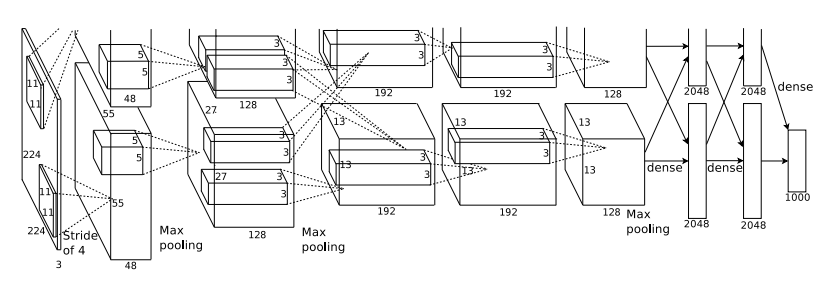
\includegraphics[width=0.8\textwidth]{assets/imgs/imagenet-cnn}
\caption{ImageNet LSVRC-2012比赛中使用的大规模卷积神经网络结构\supercite{krizhevsky2012imagenet}}
\end{figure}

% 总结
综上所述,深度学习是机器学习的全新分支,挑战了传统的机器学习方法论。神经网络通过仿生的神经元与网络设计,具象化了深度学习的特征层与堆叠方式。此外,深度学习涉及到的计算,比如卷积神经网络中的卷积层等等,都十分耗费硬件的计算资源和存储资源。本研究的主要目标即为将传统的、部署于大规模CPU和GPU的深度学习应用,运行于硬件资源和计算能力都十分有限的嵌入式平台上。接下来会对本研究涉及的硬件系统进行详细的介绍。

\section{系统芯片(SoC)}

% SoC的特点
系统芯片(System-on-Chip,简称SoC)是一类集成电路,其上包含了处理器芯片和其他电子系统,以及丰富的外部接口和设备等等。SoC主要被电子工程师用来进行系统开发和验证:SoC的处理器性能足够强大,一般足以运行常见的操作系统;SoC一般也搭载了可编程的FPGA硬件系统,可以非常方便修改硬件系统的设计。因此SoC可以明显缩短电子产品的开发周期。

% SoC的设计流程
SoC的设计分为软件与硬件两部分。软件部分的开发主要涉及偏底层的硬件驱动、数据传输、硬件控制与基于操作系统的高层次软件等等。硬件系统的设计则更加复杂:工程师一方面开发基于FPGA的硬件逻辑,定制系统所要求的特殊功能;另一方面也尽可能基于预定义的、标准的IP核(全称知识产权核,Intellectual Property core)进行基础平台的搭建,提高开发效率。此外,硬件与软件不同,在开发完成之后需要进行各种系统级、行为级的功能验证才能正式完成。正因为SoC开发难度大,目前在开发工具上和平台设计上都有相应的进展,本研究所使用的Xilinx Zynq SoC平台与SDSoC开发工具便是例证。

% SoC与嵌入式系统、研究目标的关系
本研究的目标是将深度学习框架部署于嵌入式平台中。嵌入式设备指的是一类针对特定应用场景开发的硬件设备,这类场景往往对实时性要求高,同时也对功耗与设备尺寸进行限制。SoC作为嵌入式设备的一种实现方式,完整的功能和较低的功耗比兼具,因此非常适合作为本研究的基础开发平台。第二章对本研究使用的Zynq SoC平台与SDSoC开发工具进行详细的介绍。

\section{现场可编程逻辑门阵列(FPGA)}

% FPGA可编程的特性介绍
FPGA(Field Programmable Gate Array,现场可编程逻辑门阵列)是一种特殊的半导体设备,特点在于可以对硬件逻辑进行重复编程。与ASIC(Application-Specific Integrated Circuit,专用集成电路)相比,FPGA比ASIC速度要慢,而且占用更多空间。但ASIC在设计和实现完成之后就不能修改,而FPGA可以不断修改其硬件配置,因此能大大提高硬件开发效率。与CPU相比,FPGA针对特定形式的计算速度更快,而且功耗很低,因此在嵌入式设备和SoC中往往将FPGA视为重要的组成部分。

% FPGA的组成
FPGA的基础组件为CLB(Configurable Logic Block,可配置逻辑块),其中包含LUT(Look-Up Table,查找表)、全加器和触发器(Flip-Flop)等等基本元素。CLB十分灵活,既可以用来实现时序与组合逻辑,也可以用来实现RAM。CLB之间则通过可编程的线路进行连接。FPGA的可编程性主要取决于两个部分:一个是查找表的配置,查找表中包含SRAM与多路选择器,SRAM的值随着硬件逻辑设计不同而不同,进而改变CLB的计算结果;另一个是连接CLB的线路,线路的交叉点也是可以配置进而改变CLB之间互联模式的。除此以外,不同的FPGA版本具有不同的资源配置,比如BRAM(Blocked RAM,块内存)与DSP(Digital Signal Processing,数字信号处理单元)等等在不同的FPGA上具有不同的数量,性能也不尽相同。

% FPGA的工作
传统的FPGA开发使用的是VHDL,Verilog,SystemC等硬件描述语言,这类语言用于表述硬件的寄存器传输级别(Register Transfer Level,简称RTL)的抽象。使用这类语言完成设计并仿真验证之后,便可以使用不同FPGA厂商提供的工具进行FPGA的综合(Sythesis)、实现(Implementation)和比特流生成(Bitstream Generation)。综合把电路的高级抽象转换为底层的逻辑门之间的连接,建立逻辑门网表。实现则是针对具体的FPGA硬件,进行逻辑网表的布局(Placement)、布线(Routing)以及满足资源的限制等等。最后的生成可以编程到FPGA上的比特流,比特流用来配置FPGA上的各类硬件资源。与软件编译相比,FPGA硬件的综合、实现与比特流生成往往需要花费几十分钟到数小时,依FPGA的资源和硬件设计大小而定。

% 总结
综上所述,FPGA具有可重构的硬件逻辑、优异的低功耗以及成熟的开发流程,并且广泛应用在各种计算平台中。FPGA也有其缺点,一方面是开发门槛比较高,没有数字电路基础的软件开发者很难写出性能优秀的FPGA应用;另一方面,FPGA只适用部分的计算过程,涉及到复杂的条件判断、循环等计算过程更适合部署于CPU执行。因此,本研究将FPGA作为硬件加速器,即部署计算量大但逻辑简单的计算过程于FPGA上加速。同时本研究也是用高层次综合工具提高硬件逻辑的开发效率。接下来进一步介绍高层次综合的基本概念和使用方式。

\section{高层次综合}

% 高层次综合的简介,以及优点
高层次综合(High-Level Synthesis,简称HLS)是一种将行为级的、算法级的代码转换为硬件逻辑的过程。高层次综合的输入不再是传统的硬件描述语言,取而代之的是C/C++等高级程序语言。高层次综合使得硬件逻辑开发可以从软件代码开始:传统的开发方式需要等到RTL实现完成之后才能验证,迭代周期很长;而高层次综合工具可以令开发者先实现好软件系统,之后直接把需要在FPGA上加速的代码进行高层次综合即可。通过高层次综合工具,软件工程师可以不用学习RTL级别的描述语言就可以实现硬件逻辑。根据Xilinx的调查显示,基于高层次综合的设计开发方法与传统方法相比时间加快4倍,结果质量提高0.7到1.2倍。

% 高层次综合的基本流程
一般的高层次综合流程包含如下几步:控制流和数据流图(Control Data Flow Graph)分析,资源分配(Resource Allocation),调度(Scheduling),绑定(Binding)等等。高层次综合的流程本质上是求解在资源和时间的约束下,能达到最优的资源分配和调度策略。这种最优解往往依赖启发式的算法,因此高层次综合工具分析的结果往往比较保守,在资源配置和调度上不一定能取得最佳的结果,因此需要通过开发者手动指定生成硬件的选项。比如指定某一运算需要使用DSP实现,某一循环需要流水线化等等。

% 总结
综上,高层次综合工具提供了一种生产力更高的开发FPGA应用的方式,为了取得更高的性能也需要开发者对应用进行分析、手动生成限制条件。本研究使用的SDSoC工具中整合了Xilinx Vivado HLS工具,在后续的硬件加速器的设计中主要用它进行硬件逻辑的实现和优化。

	
\chapter{使用技术}

本章阐述本研究的整体设计。整体设计部分在基本原理之上,给出更具体的实现方案设计。从本研究的目标出发,为了提供可以运行于FPGA SoC平台的深度学习框架,首先应确定用什么FPGA SoC平台和使用什么样的开发工具。其次,如果自行从头构建深度学习框架,一方面工作量过于庞大、需要考虑很多优化问题;另一方面也缺乏足够的受众,研究人员更熟悉流行的深度学习框架。因此应选用成熟的流行的深度学习框架作为基础,在其上进行针对特定嵌入式平台的适配与优化。

基于上述的考虑,本章首先介绍Xilinx Zynq平台的系统架构、搭载的ARM与FPGA的硬件特点、以及本研究使用的基于Zynq的开发板Zedboard的具体特性等等。之后给出Xilinx SDSoC工具的基本情况介绍,包括其包含的工具以及支持的开发流程。随后介绍本研究选用的基础深度学习框架Caffe,主要涉及与后续开发密切相关的软件架构和实现方式。最后,综述整体设计方案,即本研究的最终结果是如何有机结合ZYNQ,SDSoC和Caffe。

\section{Zynq平台}

Zynq平台的全称是“全可编程SoC”(All Programmable SoC)\supercite{ds190},由双核的ARM Cortex-A9处理系统(Processing System,简称PS)与Xilinx可编程逻辑(Programmable Logic,简称PL)组成。除此以外,还包含片上内存(On-chip memory),外部内存接口(External Memory Interface),各类外围设备输入输出接口(I/O Peripherals and Interfaces)以及连接PS与PL的高速AXI总线等等。

本研究基于Zynq平台的最新系列Zynq-7000进行系统设计与实现。

\subsection{Zynq系统架构}

Zynq平台的系统架构如图2.1所示。接下来分块介绍Zynq的几个组成部分。

\begin{figure}[!ht]
\centering
	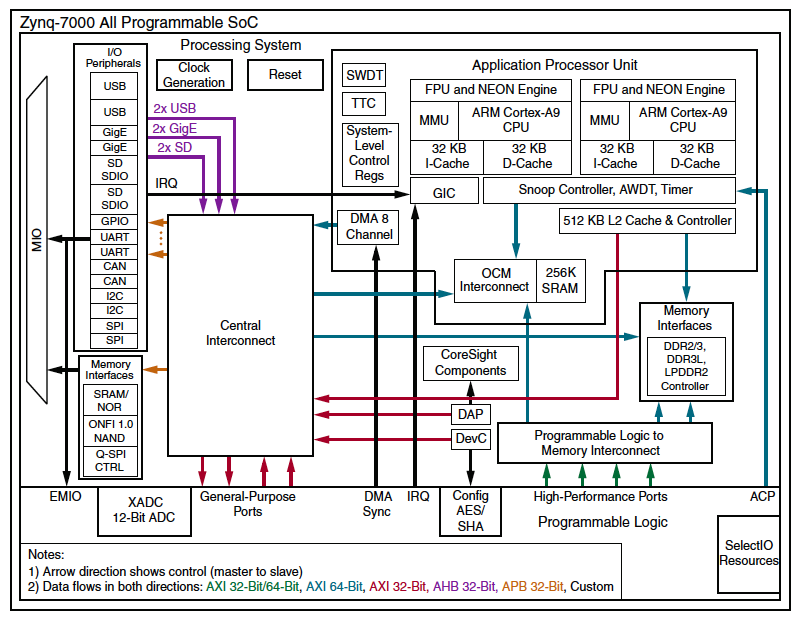
\includegraphics[width=0.8\textwidth]{assets/imgs/zynq-7000}
\caption{Zynq-7000平台的系统架构}
\end{figure}

\subsubsection{ARM处理系统}

Zynq SoC系统上搭载了双核ARM Cortex-A9 MPCore处理器,该处理器可以运行到最高1GHz,拥有指令和数据的32KB L1缓存与512KB L2缓存,以及NEON媒体处理引擎(media-processing engine)和浮点数向量处理单元(Vector Floating Point Unit,简称VFPU)等等。Cortex-A9的性能十分优异,足以满足多种情况下的计算需求。

本研究中依赖该ARM处理器提供的CPU端环境进行大部分的计算。有关ARM处理器与内存系统和PL的交互接口在2.1.4节介绍。

\subsubsection{可编程逻辑}

Zynq的可编程逻辑(PL)与一般的FPGA设计一致,主要包含CLB,BRAM以及DSP处理单元。相关指标如下表所示:

\begin{table}[!ht]
\centering
\begin{tabular}{ | l | l | l | l | l | }
\hline
Logic Cells & LUTs & Flip-Flops & BRAMs & DSP Slices \\ \hline
85K & 53,200 & 106,400 & 560 KB & 220 \\
\hline
\end{tabular}
\caption{Zynq-7000 XC7Z020可编程逻辑上资源容量}
\end{table}

本研究使用的XC7Z020系列Zynq的可编程逻辑的配置与性能大致上与Artix-7 FPGA相似,硬件资源比较有限。因此想要取得高效的性能必须做精细的资源分配和优化。相关的优化策略和技巧在第四章详述。

\subsubsection{数据通路AXI与存储系统}

存储系统与数据通路负责连接处理系统与可编程逻辑,以及处理和其他外围设备通信。Zynq平台的存储系统主要由三个部分组成:处理系统中的缓存(L1与L2 cache)和片上内存(On-chip Memory);可编程逻辑上的BRAM;以及大容量的外部存储(External Memory)。Zynq上的几种数据通路可以完成这三个组成部分之间的不同形式的交互。

Zynq上的数据通路的基础是ARM的AXI(Advanced eXtensible Interface)\supercite{ug761}总线协议,属于AMBA(Advanced Microcontroller Bus Architecture)协议的一部分。
AXI的最新版本是AXI4协议,Xilinx设计并实现了基于AXI4的IP核,使得AXI变得更加灵活、高效和便捷。AXI4协议主要有三类:针对大数据量传输的AXI4,小数据量的AXI4-Lite,以及针对流数据的AXI4-Stream。Zynq上的数据通路正是基于Xilinx提供的AXI IP核实现的。

Zynq基于AXI总线协议连接处理系统和可编程逻辑,主要实现两类接口:高性能AXI端口(High-Performance AXI ports)与ACP(Accelerator Coherency Port)接口,二者区别关键在内存数据一致性上。高性能AXI端口可以实现处理系统和可编程逻辑高速的数据传输,但不保证CPU缓存中的数据与内存读写一致。ACP接口则在硬件机制上保证缓存中的数据在传输之前被写回内存、内存更新之后缓存同步更新。

在设计Zynq应用时具体使用哪种数据通路取决于系统的特性。本研究在第三章给出对数据通路选择的原则,在第四章会具体讨论两种数据通路的性能对比。

\subsection{Linux运行模式}
基于Zynq平台开发的应用有两种运行模式:Standalone与Linux模式。前者代表应用的运行不用启动操作系统,后者则要求先启动Linux操作系统再运行应用。考虑到深度学习应用并不是简单的计算,还需要各种数据处理的操作,并且科研人员更熟悉基于操作系统的运行模式,本研究只在Linux模式下进行开发。

Linux模式首先启动预先加载与ROM中的引导程序,该程序从SD卡中读取第一阶段启动程序(First Stage Boot Loader, 简称FSBL),FSBL负责处理可编程逻辑的比特流(bitstream)和Linux引导程序(u-boot)的加载与执行。引导程序之后分别加载Linux的镜像文件(uImage)、设备树文件(Device Tree)和根系统文件(Rootfs)。Linux镜像主要包含Linux内核,设备树文件定义了硬件设备环境供引导程序动态加载,根系统文件则包含了系统的根目录和必要的程序与库。准备就绪之后即可通过UART接口或者SSH连接到Zynq平台,运行程序或进行开发。

Xilinx提供了bootgen工具来创建SD卡引导程序,以及一系列预生成的文件,例如Linux镜像,根系统文件等等。SDSoC工具中包含了bootgen,以及更多跟硬件平台相关的预生成文件,可以更简便地生成SD卡中需要的内容。在2.3节中会进一步介绍。

\subsection{Zedboard}
本研究选用的是Zedboard作为Zynq开发平台。Zedboard\supercite{zed}是基于Zynq-7000系列的扩展式处理平台,Zedboard上除了满足Zynq-7000所要求的ARM Cortex-A9 MPCore处理器与Xilinx FPGA之外,还增加了如下配置:512MB DDR3内存、256MB QSPI闪存和一系列输入输出接口(HDMI、VGA、OLED与音频接口)等等。除此以外,Zedboard成本低廉,还有Xilinx SDSoC的特别支持,尤其是预先搭载好的输入输出接口对深度学习应用的开发(计算机视觉等应用)非常方便。因此本研究使用Zedboard作为最终深度学习框架所运行的平台。

\section{SDSoC开发环境}

Xilinx于2015年3月推出了SDSoC开发环境,提供类似于嵌入式C/C++开发体验。SD即“软件定义”(Software Defined)\supercite{sdsoc}:
SDSoC的目标是降低FPGA应用开发门槛,让更多的软件开发者,而不是专业的FPGA开发人员,可以通过C/C++代码直接生成Zynq SoC系统。此外,SDSoC综合了Vivado HLS,Xilinx ARM GNU编译工具链,以及一系列系统生成工具(bootgen, Xillybus等等),令开发效率得到很大提升。但是SDSoC的最大优势在于其对传统SoC开发流程的改进。接下来主要介绍SDSoC的开发流程与基本使用方式。

\begin{figure}[!ht]
\centering
	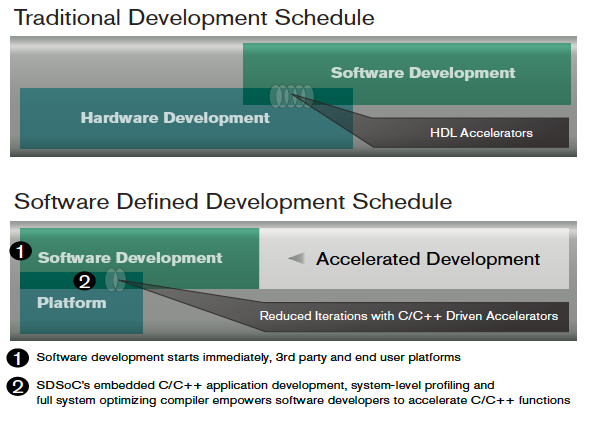
\includegraphics[width=0.7\textwidth]{assets/imgs/software-defined}
\caption{传统的开发流程(Traditional Development Schedule)与软件定义的开发流程(Software Defined Development Schedule)的区别}
\end{figure}

\subsection{软件定义的开发流程}

传统的SoC平台的系统开发流程首先需要完成硬件部分的设计,之后软件开发者才能通过已经综合实现好的硬件接口进行进一步开发。这种开发流程迭代周期非常长,软件部分的开发在硬件设计过程中处于停滞状态,硬件设计只能等软件部分完成才能获得反馈。基于SDSoC的开发基于软件定义的开发流程:先用C/C++代码完成整个系统的设计,之后以函数为单元部署于可编程逻辑,进行硬件加速。SDSoC甚至提供了硬件加速性能预测工具,可以令开发人员在长时间的综合实现完成之前就能大概了解目前的优化策略是否正确。图2.2是对两种开发流程的对比。

\subsection{基本概念与使用方式}

\subsubsection{数据移动网络}
SDSoC开发环境关键概念是数据移动网络(data motion network)\supercite{ug1027},
表示PS与PL之间的数据通路模式:SDSoC使用预先设计好的数据通路IP核来负责PS与PL之间的数据传输,这些IP核称为数据移动单元(data mover)。比如AXIDMA\_SG就表示通过AXI总线用Scatter-Getter的方式通过DMA传输数据。数据移动单元与数据类型密切相关,标量数据只能用AXI\_LITE传输,而数组与更复杂的数据类型可以用AXI\_DMA\_SG,AXI\_DMA\_SIMPLE,AXI\_DMA\_2D等数据传输单元传输。一般而言SDSoC可以根据数据类型,内存分配方式等分析出最适合使用的数据传输单元,但开发者也可以使用预编译指令(pragma)进行优化。

\begin{figure}[!ht]
\centering
	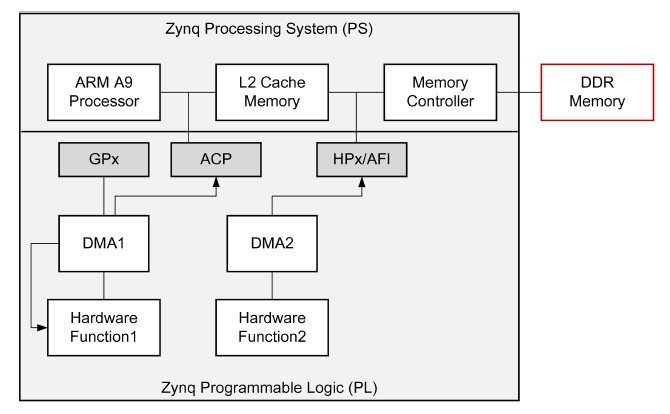
\includegraphics[width=0.8\textwidth]{assets/imgs/zynq-axi}
\caption{Zynq AXI总线协议的几种端口}
\end{figure}

\subsubsection{使用方式}
SDSoC的可以通过其IDE使用,也可以基于纯粹的Linux命令行使用。由于IDE的限制更多,本研究完全使用命令行环境开发。SDSoC的最关键工具是sdscc/sds++。这两个程序本质上为C/C++编译器,可以完全兼容gcc/g++的命令行选项。但与一般编译器不同,sdscc/sds++可以通过命令行选项指定:1)需要HLS的函数:包含函数名和要求的时钟频率;2)数据移动网络的时钟频率;3)目标硬件平台:比如zed(针对Zedboard)或zybo(针对ZYBO开发板)。因此,通过sdscc/sds++工具可以轻易与原有的Linux项目进行兼容。有时候也需要更细粒度的操作,可以使用arm-xilinx-linux-gnueabi的GNU工具链对C/C++代码进行交叉编译,使用sdslib封装IP核等等,在第三章对Caffe和第三方库的移植中会详细介绍。

本研究的应用完全依赖SDSoC进行开发,利用Vivado HLS进行硬件逻辑编写和优化,SDSoC自带的IP核进行数据通路的自动生成,以及Xilinx ARM GNU工具链编译CPU端代码并进行链接。最后SDSoC把项目全部整合到SD卡中。

\section{深度学习框架Caffe}

Caffe\supercite{jia2014caffe}是加州伯克利大学计算机视觉与学习中心\footnote{Berkeley Vision and Learning Center,\url{http://bvlc.eecs.berkeley.edu/}}开发的深度学习框架,基于C++与CUDA开发。Caffe因其速度快,数据模版清晰易懂,并拥有开源的、高度模块化的代码而广受开发者欢迎。

本研究选用Caffe作为移植到Zynq上进行移植和加速的对象,主要是因为其清晰的软件架构,非常便于修改和优化。除此以外,与其他深度学习框架(如基于LuaJIT的Torch,基于Python的Theano)相比,Caffe的CPU端代码完全基于C++实现,与高层次综合工具、ARM GNU编译工具链、SDSoC等等可以无缝衔接。因此本研究最终选用Caffe作为优化的基础。

接下来首先介绍Caffe的使用中出现的关键概念,之后着重介绍与移植相关的Caffe软件架构和神经网络层的实现。

\subsection{基本概念}
Caffe中的网络层Layer和网络Net是两个关键概念。Caffe Layer是对神经网络层的抽象,通过指定使用的预定义网络类型,上下层连接的网络名称,以及本层的参数就可以构建一个Caffe Layer。Caffe Layer之间连接起来的有向无环图(Directed Acyclic Graph,简称DAG)便是Caffe Net,即神经网络。Caffe的神经网络训练是用Caffe Solver(求解器)实现的,一个Caffe Solver中定义了训练的网络名称、控制训练的参数以及运行的硬件(CPU或GPU)等等。Caffe Layer、Caffe Net和Caffe Solver都可以使用Google Protocol Buffer\footnote{Google Protocol Buffer (\url{https://developers.google.com/protocol-buffers/docs/overview})不仅提供了一种接口数据传输的格式,同时还可以生成数据传输与序列化的代码。}文档格式进行定义。

从具体实现的角度出发,理解Caffe的代码关键需要理解Layer类和Blob类。每个Caffe的Layer类都实现了Forward与Backward两个方法,相当于神经网络中的前向与反向计算。Forward与Backward的两个参数都是用Blob类表示的网络层输入输出。Blob类本质上是多维数组,因此可以处理各种形状的网络层输入输出。

Caffe的标准用法有两种,一种是通过编译出的caffe命令行工具直接训练Caffe模型,其中Caffe模型与训练数据需要提前定义好;除此以外,也可以使用Caffe动态链接库(libcaffe.so)在其他的C++应用中使用Caffe提供的接口。两种方法都十分方便。

\subsection{软件架构}
% 这一部分之后需要进一步扩充,主要是面向对象设计的部分:Blob类是什么,Net和Layer类是什么等等
Caffe的软件架构主要包含如下几个部分,依赖关系具有清晰的分层次的结构:
\begin{enumerate}
\item 基础架构:数据类型的定义,比如blob.cpp定义了Blob数据结构,net.cpp与layer.cpp分别定义了网络类与网络层类。同时常用数学函数math\_functions.cpp也十分重要,Caffe的各种大运算量的计算基本都会调用该文件所定义的函数。
\item 网络层的实现:在layers/目录下定义了常见的神经网络层的实现,比如卷积神经网络conv\_layer.cpp,ReLU层relu\_layer.cpp等等。相关GPU代码也包含其中。
\item 求解器实现:在solvers/目录下定义了多种求解器,比如SGD求解算法。
\item 其他:比如Caffe使用的Protobuf文件等等。
\end{enumerate}

\subsection{第三方库依赖}
Caffe所依赖的第三方库不多,可以简单分为如下几类:
\begin{enumerate}
\item 数据存储:
Caffe使用LMDB\footnote{即Lightning Memory-Mapped Database,提供键值存储,使用B+Tree实现。\url{https://symas.com/products/lightning-memory-mapped-database/}}与
LevelDB\footnote{LevelDB也是一个轻量的存储库,由Google开发,使用LSM树算法\url{(http://leveldb.org/)}}两种存储形式对数据进行保存。
\item 数据格式和接口:
HDF5\footnote{HDF5主要用来定义复杂的数据模型\url{https://www.hdfgroup.org/HDF5/}}与Protobuf
\item 数学计算:BLAS运算库
\item 其他:比如日志、基础组件等等
\end{enumerate}

总之,Caffe的分层设计和简单的第三方库依赖都非常便于优化和修改。本研究针对Caffe的移植与优化在第三章中详述。



	\chapter{主体工作}

从上述整体设计出发,本研究的主要实现了SoCaffe — 一个基于深度学习框架Caffe并能运行于任一基于Zynq架构的嵌入式SoC设备上的深度学习框架。SoCaffe的名称来源于SoC与Caffe的结合。

本研究的主体工作可以分为如下三步:
\begin{enumerate}
\item 系统分析与架构设计:划分Caffe在SoC上的软硬件职责,确定CPU运行和FPGA加速的部分;
\item FPGA加速器实现:实现硬件逻辑与应用优化策略;
\item ARM系统实现:构建数据通路、综合编译软硬件系统;
\end{enumerate}

本研究的最终成果包含编译好的基于FPGA的硬件加速库、使用硬件加速的Caffe链接库以及全部依赖的第三方链接库。使用本研究提供的Caffe版本与动态链接库,便可以直接实现基于Zynq SoC的深度学习应用。本研究的主体工作完全基于SDSoC工具实现:FPGA加速器使用了SDSoC包含的Vivado HLS工具进行硬件逻辑的编写与优化;数据通路构建依赖SDSoC提供的数据接口IP库;ARM系统的综合编译依赖SDSoC提供的ARM GNU编译工具链。

接下来按步骤介绍主体工作。

\section{系统分析与架构设计}

% Caffe的软硬件划分思路
只用ARM CPU完全足以运行Caffe,但性能不尽如人意。SoC上的CPU本身计算性能有限,而且难以并行化,因此需要FPGA硬件进行部分计算的硬件加速。由于GPU与FPGA在高性能计算的应用中拥有类似的特性,因此可以从Caffe的GPU加速函数中进行筛选,选择最适合FPGA计算的函数进行硬件加速。筛选的原则主要有以下三条:1)函数需要拥有较长的计算时间,占据总运行时间的很大比重,根据阿姆达尔定律(Amdahl's Law)加速类函数可以取得最大的加速比;2)代码逻辑简单,并行度高,适合在FPGA上运行;3)数据传输量小,不会花费很多时间在FPGA与CPU之间的数据传输上。从上述角度出发,本研究选用GEMM(GEneral Matrix Multiplicaion,通用矩阵乘法)作为在FPGA上主要优化的目标函数。

% GEMM简介
GEMM计算属于BLAS(Basic Linear Algebra Subprograms,基本线性代数子程序)集合,结合了矩阵乘法与加法计算:
\begin{equation}\label{eq:gemm}
\mathbf{C} \leftarrow \alpha op(\mathbf{A})op(\mathbf{B}) + \beta \mathbf{C}
\end{equation}

$\mathbf{A}$,$\mathbf{B}$,$\mathbf{C}$分别是输入矩阵,$\alpha$与$\beta$分别为GEMM计算的系数。此外,$op$函数会随着配置不同,对输入矩阵$\mathbf{A}$与$\mathbf{B}$不变换或者进行转置变换。因此GEMM具有充分的灵活性,可以配置出各种形式的矩阵乘法与加法组合。

% Caffe中对GEMM的使用
Caffe中大量使用了GEMM计算,主要在网络层的计算过程中,比如卷积层的卷积计算(\texttt{conv\_layer.cpp})。Caffe计算卷积的策略是把复杂的卷积操作变为简单的矩阵乘法问题,进而可以使用效率更高的、充分优化过的BLAS计算库。变换的方法主要是使用im2col操作对原始输入矩阵进行变换,把分离的矩阵块聚合起来\footnote{Caffe的作者贾扬清(Yangqing Jia)在这篇文章中解释了Caffe是如何使用GEMM与im2col来实现卷积层的:\url{https://github.com/Yangqing/caffe/wiki/Convolution-in-Caffe:-a-memo}}。总之,Caffe通过GEMM实现的卷积操作取得了不错的优化效果。

综上,整个深度学习框架在SoC上的划分如图3.1所示。处理系统上运行深度学习应用,并链接第三方链接库(比如OpenBLAS、LMDB等等)、caffe链接库(\texttt{libcaffe.so})与加速器链接库(\texttt{libaccel.so})。硬件加速器链接库提供调用FPGA硬件逻辑的高层接口。FPGA上主要实现了GEMM计算的硬件逻辑。PS与FPGA之间通过AXI总线和内存进行数据交互。
\begin{figure}[!ht]
\centering
	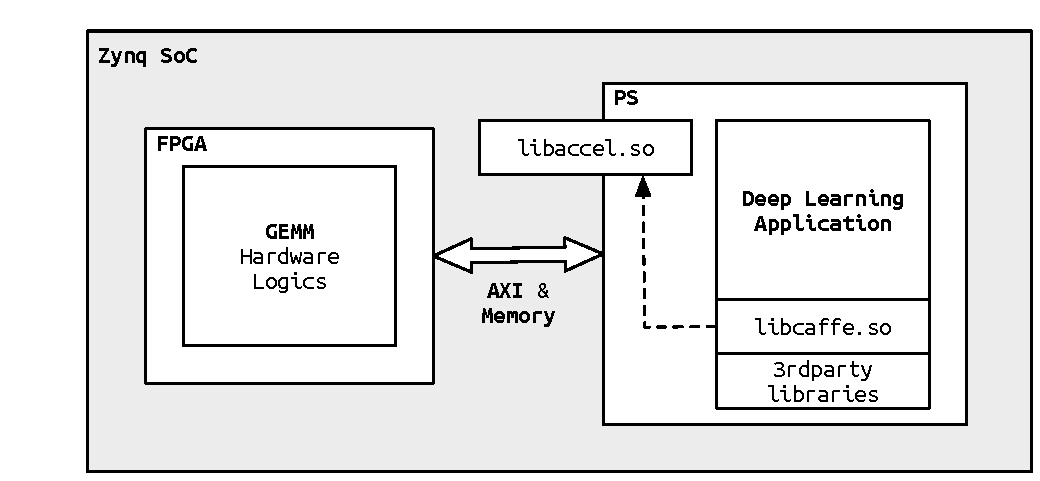
\includegraphics[width=0.9\textwidth]{assets/imgs/socaffe}
\caption{SoCaffe的系统架构}
\label{fig:socaffe}
\end{figure}

接下来分别介绍FPGA的加速器实现与ARM处理系统的实现工作。

\section{FPGA加速器实现}

基于FPGA实现的GEMM加速器是本研究的关键工作。本研究使用Vivado HLS工具设计并实现了基于固定大小的矩阵块之间的GEMM计算,并使用多种资源分配和调度策略进行优化;处理系统与FPGA之间的数据通路使用SDSoC工具提供的IP核实现;最后通过链接使得Caffe可以使用GEMM加速器进行计算。整个GEMM加速器基本使用了全部的FPGA硬件资源,相对于运行于CPU上的OpenBLAS库有5.45x倍速度提升,相应的测试结果在第四章详述。

\subsection{GEMM实现}

% GEMM算法特性的介绍
GEMM本身并不复杂,以传统的三重循环实现的矩阵乘法为基础就可以在CPU上实现。下面的算法中以矩阵$\mathbf{C}$的行、列为优先,假设每次迭代的坐标为$(i,j)$。每次迭代首先把$\beta \times \mathbf{C}(i,j)$作为累积变量$sum$的初值,进而遍历矩阵$\mathbf{A}$和$\mathbf{B}$的$i$行与$j$列(如果$\mathbf{A}$或$\mathbf{B}$需要转置则使用$i$列或$j$行,算法的5、6行使用了C语言的三元条件表达式表示转置条件),将$\mathbf{A}$与$\mathbf{B}$的对应元素和$\alpha$相乘并累加。最后把$sum$赋给$\mathbf{C}(i,j)$。


\begin{algorithm}
\caption{GEMM的原始三重循环算法}
\label{alg1}
\algsetup{indent=2em}
\begin{algorithmic}[1]
\FOR{$i=0$ \TO $M$}
  \FOR{$j=0$ \TO $N$}
    \STATE{$sum \leftarrow \beta \times \mathtt{C[i][j]}$}
    \FOR{$k=0$ \TO $K$}
      \STATE{$a \leftarrow \mathtt{(TA)\ ?\ A[i][k]\ :\ A[k][i]}$}
      \STATE{$b \leftarrow \mathtt{(TB)\ ?\ B[k][j]\ :\ B[j][k]}$}
      \STATE{$sum \leftarrow \alpha \times a \times b$} 
    \ENDFOR
    \STATE{$\mathtt{C[i][j]} \leftarrow sum$}
  \ENDFOR
\ENDFOR
\end{algorithmic}
\end{algorithm}


\subsubsection{GEMM分块矩阵算法}
% 分块的原理
如果要将该算法移植到FPGA上,首先需要对矩阵计算进行分块。FPGA上只有有限的硬件资源,而且在计算开始之前已经固定,所以不可能进行使用该算法在FPGA上计算任意大小的矩阵。所谓分块(tiling),是指将原先以矩阵元素为单元的遍历方式,改变为以固定大小的矩阵块为单元的遍历方式。分块矩阵算法的基本原理是分块矩阵乘法与分块矩阵转置的计算公式(如图3.2,3.3)。

\begin{figure}[!ht]
\[
\begin{pmatrix}
  A_{1,1} & A_{1,2} & \cdots & A_{1,k} \\
  A_{2,1} & A_{2,2} & \cdots & A_{2,k} \\
  \vdots  & \vdots  & \ddots & \vdots  \\
  A_{m,1} & A_{m,2} & \cdots & A_{m,k} 
\end{pmatrix}
\times
\begin{pmatrix}
  B_{1,1} & B_{1,2} & \cdots & B_{1,n} \\
  B_{2,1} & B_{2,2} & \cdots & B_{2,n} \\
  \vdots  & \vdots  & \ddots & \vdots  \\
  B_{k,1} & B_{k,2} & \cdots & B_{k,n} 
\end{pmatrix}
=
\begin{pmatrix}
  C_{1,1} & C_{1,2} & \cdots & C_{1,n} \\
  C_{2,1} & C_{2,2} & \cdots & C_{2,n} \\
  \vdots  & \vdots  & \ddots & \vdots  \\
  C_{m,1} & C_{m,2} & \cdots & C_{m,n} 
\end{pmatrix}
\]

\caption{分块矩阵的乘法运算}
\end{figure}
\begin{figure}[!ht]
\[
\begin{pmatrix}
  A_{1,1} & A_{1,2} & \cdots & A_{1,k} \\
  A_{2,1} & A_{2,2} & \cdots & A_{2,k} \\
  \vdots  & \vdots  & \ddots & \vdots  \\
  A_{m,1} & A_{m,2} & \cdots & A_{m,k} 
\end{pmatrix}^T
=
\begin{pmatrix}
  A_{1,1}^T & A_{2,1}^T & \cdots & A_{m,1}^T \\
  A_{1,2}^T & A_{2,2}^T & \cdots & A_{m,2}^T \\
  \vdots    & \vdots    & \ddots & \vdots    \\
  A_{1,k}^T & A_{2,k}^T & \cdots & A_{m,k}^T 
\end{pmatrix}
\]

\caption{分块矩阵的转置运算}
\end{figure}

上述公式中的矩阵元素都是矩阵块,每个矩阵中的矩阵块大小一致。$m$,$n$,$k$分别为按照块大小划分后的矩阵中块的个数。分块矩阵乘法运算的结果中,每个结果矩阵块都是由块之间的乘法和累加构成的:
$$\mathbf{C}_{i,j}=\sum_{t=0}^{k} \mathbf{A}_{i,t} \times \mathbf{B}_{t,j}$$

而分块矩阵转置运算的结果相当于先以矩阵块为单元进行转置,之后分别对每个矩阵块进行内部转置。

从上述两个公式出发便可以得到GEMM的分块矩阵算法。$BLK\_M$,$BLK\_N$,$BLK\_K$分别为矩阵的块尺寸参数。本算法的框架基本与GEMM原始算法类似,但是其中计算参数都是矩阵块而不是矩阵元素。

\begin{algorithm}
\caption{GEMM的分块矩阵算法}
\begin{algorithmic}[1]
\FOR{$bi = 0$ \TO $\lceil M/BLK\_M \rceil$}
  \FOR{$bj = 0$ \TO $\lceil N/BLK\_N \rceil$}
    \STATE{$\mathbf{S} \leftarrow \beta \times \mathbf{C}_{bi,bj}$}   
    \FOR{$bk = 0$ \TO $\lceil K/BLK\_K \rceil$}
      \STATE{$\mathbf{A}_b \leftarrow \mathbf{A}_{bi,bk}$ or transposed $\mathbf{A}_{bk,bi}^T$}
      \STATE{$\mathbf{B}_b \leftarrow \mathbf{B}_{bk,bj}$ or transposed $\mathbf{B}_{bj,bk}^T$}
      \STATE{$\mathbf{S} \leftarrow \alpha \times \mathbf{A}_b \times \mathbf{B}_b + \mathbf{S}$}
    \ENDFOR
    \STATE{$\mathbf{C}_{bi,bj} \leftarrow \mathbf{S}$}
  \ENDFOR
\ENDFOR
\end{algorithmic}
\end{algorithm}


接下来具体介绍如何把分块矩阵算法实现于FPGA上。

\subsubsection{硬件加速实现}\label{subsubsec:normal}

FPGA上主要加速的是GEMM分块矩阵算法的第7行,对两个固定大小的矩阵块求乘法并进行累加。因此,矩阵块的大小不能任意取值,主要受限于FPGA的硬件资源数量:越大的矩阵需要越多的板上计算资源和存储资源。此外,为了适配Caffe的接口,该算法主要针对单精度浮点数格式设计实现。最后,为了简化FPGA实现的接口,CPU端会分配几个固定大小的矩阵块用来保存传输到硬件的参数。

\begin{figure}[!ht]
\centering
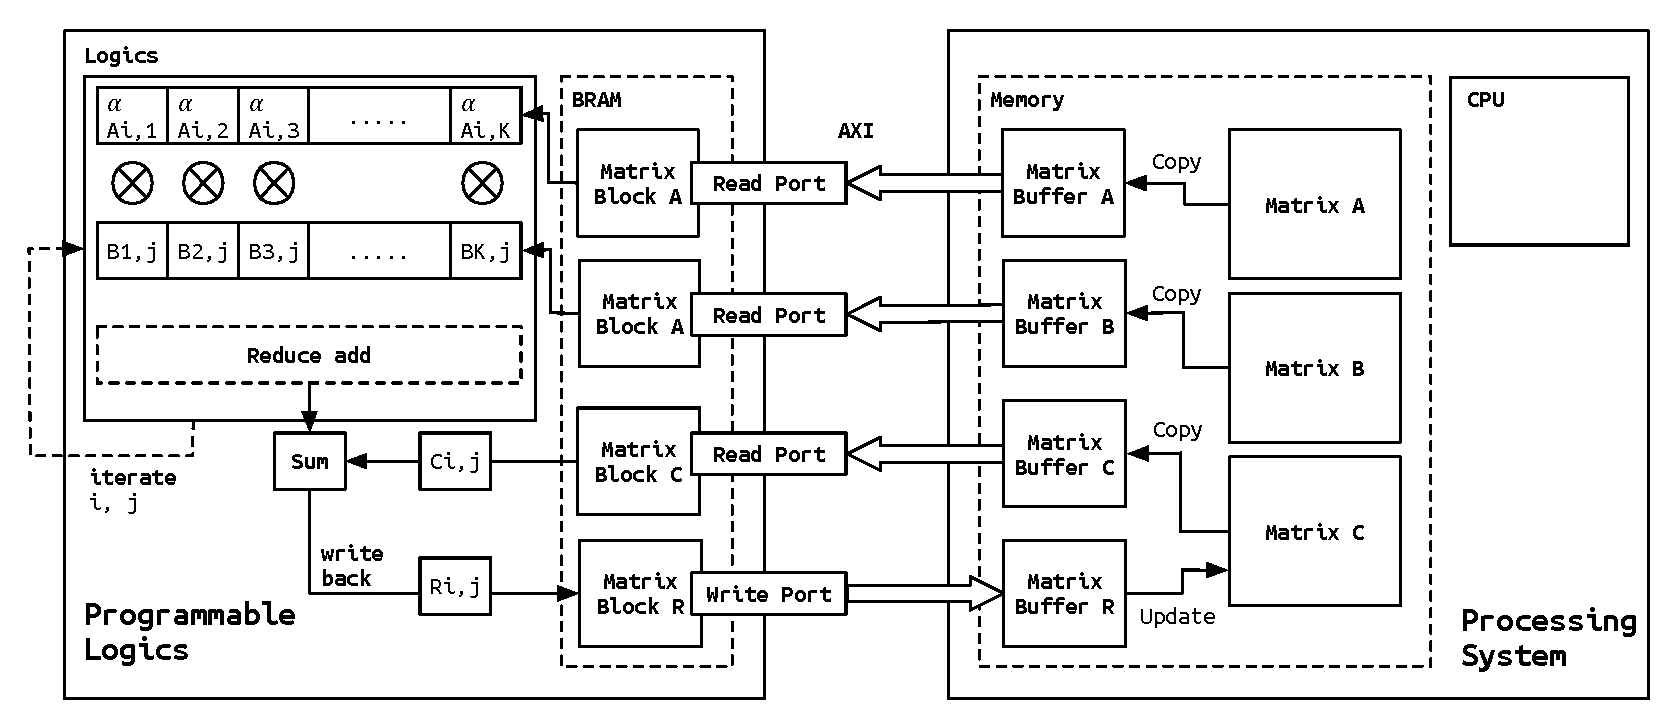
\includegraphics[width=\textwidth]{assets/imgs/gemm}
\caption{GEMM的软硬件设计}
\end{figure}

图3.4是具体的硬件加速设计架构:左侧为FPGA可编程逻辑,右侧为处理系统,二者之间通过AXI总线通信。如图所示,每次计算会先从矩阵中复制矩阵块到专门划分的缓存区中,如果有需要转置则在复制过程中进行转置(如算法2的第5,6行)。之后,FPGA把缓存的矩阵块放入BRAM中,在每个迭代步都进行矩阵乘法运算中的点积操作。矩阵$\mathbf{C}$也被读入,和点积结果进行累加。FPGA上的数据写回到矩阵$\mathbf{R}$中,防止与对$\mathbf{C}$的访问冲突。当计算完成之后,处理系统使用矩阵$\mathbf{R}$的结果对内存中的矩阵$\mathbf{C}$进行更新,每次更新一个矩阵块大小的数据。

上述GEMM加速系统的设计的软件端代码可以很容易地实现,但是硬件端代码主要有两部分组成:将总线中的数据复制到BRAM,以及从BRAM中读取数据进行计算。硬件逻辑代码如代码\ref{lst:gemmaccel}和代码\ref{lst:gemmaccelkern}所示。
\begin{listing}[!ht]
\inputminted[
  mathescape, 
  linenos,
  numbersep=5pt,
  breaklines=true,
  fontsize=\footnotesize]{c}{assets/codes/hls.c}

\caption{\texttt{gemm\_accel}函数的定义(未优化)}
\label{lst:gemmaccel}
\end{listing}

\begin{listing}[!ht]
\inputminted[
  mathescape, 
  linenos,
  numbersep=5pt,
  breaklines=true,
  fontsize=\footnotesize]{c}{assets/codes/hlskern.c}
\caption{\texttt{gemm\_accel\_kernel}函数的定义(未优化)}
\label{lst:gemmaccelkern}
\end{listing}

% 简单介绍代码的情况
这两份代码都默认矩阵块的大小必须完全相同,这是一种简化,在实际实现的代码中尺寸可以不一致。\texttt{gemm\_accel}是被指定为要被HLS生成硬件的函数,因此\texttt{Ab},\texttt{Bb}与\texttt{Cb}都会被实现为FPGA上的BRAM\footnote{有的时候HLS工具也会用LUT来生成存储,选择BRAM还是LUT可以在程序中显式指定},\texttt{gemm\_accel}所调用的\texttt{gemm\_accel\_kernel}中的计算过程也会被实现为硬件逻辑。

\subsubsection{基本优化技巧}
两个函数中出现的循环一般会被实现为硬件逐步迭代进行的计算,但因为在代码中使用HLS的流水线预编译指令(pipeline),因此循环的迭代步之间可以同时执行:上一步迭代的计算与这一步迭代的BRAM读取不冲突,可以并行。流水线化是实现高效硬件逻辑的关键步骤,在Vivado HLS工具中,流水线化与循环控制流密切相关,被流水线化的循环内部的嵌套循环会被默认进行循环展开(Loop Unrolling)。同时,初始化间隔(Initialization Interval,简称II)指的是流水线需要几个时钟周期才能进行初始化,当II=1时流水线化达到最佳水平。II=1的结果主要因为对A和B的数组划分(Array partition):对A与B的访问可以同时通过多个端口进行,这样流水线便不会阻塞。

\begin{table}[!ht]
	\centering	
	\begin{tabular}{ | l | l | l | l | l |}
		\hline
		BRAM\_18K (\%) & DSP48E (\%) & FF (\%) & LUT (\%) & Latency (cycles) \\ \hline
		23 & 72 & 18 & 46 & 2352 \\ \hline
	\end{tabular}
	\caption{当前代码的HLS结果,包含资源占用率与预测延迟}
	\label{table:gemmorig}
\end{table}

对上述代码进行高层次综合可以得到一份简单的报告,进而可以分析得到当前代码的理论效率与资源占用情况。表\ref{table:gemmorig}是针对上述算法综合的$\mathtt{Dim}=32$的GEMM计算硬件资源占用。

% 性能预测与高层次综合报告
\subsection{GEMM性能分析与预测}

% 前提假设
本节从GEMM算法的特性出发,找出性能与GEMM分块算法中的块大小之间的数学关系。性能指标的单位为GFLOPS(Giga floating-point operations per second,每秒1G次浮点运算操作个数)。由于GEMM分块算法有多种分块方式,为了简便起见本节中使用正方形划分的分块方式,即从矩阵$\mathbf{A}$,$\mathbf{B}$,$\mathbf{C}$划分出的任意块$\mathbf{A_{ik}}$,$\mathbf{B_{jk}}$与$\mathbf{C_{ij}}$都是正方形。此外,本节性能分析只涉及FPGA硬件逻辑的计算时间,数据传输延迟暂不考虑。

% FPGA的性能预测概论
理论上,FPGA的运行时间($time_{HW}$)延迟($latency$,单位为时钟周期数)和时钟频率($freq$,单位为MHz)相关:

\begin{equation}\label{eq:timelatency}
time_{HW}=\frac{latency}{freq}
\end{equation}
% $$\mathtt{time} = \mathtt{latency} \times 1 / \mathtt{frequency} = 2352 / (143 \times 10^{6}) s = 1.64 s$$

% 延迟大小与GEMM块大小的关系
延迟的大小与GEMM使用的矩阵块大小密切相关。矩阵块大小由三个参数决定:$Dim_M$,$Dim_N$,$Dim_K$\footnote{$M$,$N$,$K$的语义与描述矩阵乘法的场景中使用的语义一致,即$Dim_M$为矩阵块$\mathbf{A_{ij}}$的高,$Dim_K$为其宽。其余可以类推得到。}。
原始实现(如\ref{subsubsec:normal}节所示)中延迟由两个子过程决定,分别为BRAM复制与GEMM计算。
% BRAM复制与GEMM块大小的关系
BRAM复制过程包含三个独立的、流水线化的循环,总延迟(\(\mathit{L_{BRAM}}\))等于三个循环的延迟之和。
假设初始化间隔已经达到目标1,则流水线化的循环延迟约等于循环体的延迟\footnote{\(\mathbf{A}\)矩阵块的BRAM复制循环与其他循环不同,延迟主要取决于与\(\alpha\)的乘法计算延迟,因为乘法比赋值更慢}加上循环周期数,因此:
\begin{equation}\label{eq:bramcopylatency}
\begin{aligned}
\mathit{L_{BRAM}}
& = \mathit{L_{AMultLoop}+L_{BCopyLoop}+L_{CCopyLoop}} \\
& = \mathit{Dim_M\times Dim_K + L_{mult}} 
  + \mathit{Dim_N\times Dim_K + L_{copy}} \\
& + \mathit{Dim_M\times Dim_N + L_{copy}} \\
& = \mathit{S_A + S_B + S_C + 2L_{copy} + L_{mult}} 
\end{aligned}
\end{equation}
%对于固定大小矩阵块的GEMM计算而言,一次运算共进行$\mathtt{Dim}^3\times2+\mathtt{Dim}^2+\mathtt{Dim}^2\times 2 = 2\mathtt{Dim}^3+3\mathtt{Dim}^2$次浮点数运算。因此理论上GFLOPS(每秒G次浮点数运算)的结果为:
%$$\mathtt{GFLOPS} = (2\mathtt{Dim}^3+3\mathtt{Dim}^2)/\mathtt{time} = 4.17$$
即BRAM复制过程的延迟等于三个矩阵块的面积和与两个复制的延迟(\(\mathit{L_{copy}}\))、一个乘法运算的延迟(\(\mathit{L_{mult}}\))的和。
% 乘法计算与GEMM块大小的关系
GEMM计算延迟(\(\mathit{L_{comp}}\))取决于流水线化的GEMM三重循环计算,由于其中第二层循环被流水线化,这部分的总延迟等于前两层的循环周期数加上第三层循环完全展开后的点积计算延迟(\(\mathit{L_{prod}}\)):
\begin{equation}\label{eq:complatency}
\begin{aligned}
\mathit{L_{comp}}
& = \mathit{Dim_M \times Dim_N + L_{prod}} \\
& = \mathit{S_C + Dim_K \times L_{add} + L_{others}}
\end{aligned}
\end{equation}
简单对数据流进行分析可以发现,由于点积运算中包含存在依赖的求和运算,且这部分的延迟与\(\mathit{Dim_K}\)成正比
\footnote{根据\cite{ug902}第183页,对于浮点数格式的加法,为了防止出现精度问题,不会使用平衡过的加法树(Adder Tree),因此延迟与\(Dim_K\)的关系是线性而不是对数的。}
,因此GEMM计算延迟与\(\mathit{Dim_K}\)相关。

% 总延迟
综上,假定矩阵块面积的大小是主要决定因素(其他延迟变量的值暂且忽略不计),且令\(\mathit{Dim}\)为最大矩阵块尺寸,则综合公式\ref{eq:bramcopylatency}与\ref{eq:complatency},得到总延迟的表达式为:
\begin{equation}\label{eq:latency}
\begin{aligned}
\mathit{latency} 
& = \mathit{L_{BRAM}} + \mathit{L_{comp}} \\
& \approx \mathit{S_A + S_B + 2S_C} \leq 4Dim^2
\end{aligned}
\end{equation}
即总延迟的大小的上界为\(\mathit{4Dim^2}\)。

% 总浮点数操作数
GEMM的浮点数操作数总数(\(\mathit{FLOP}\))也取决与矩阵块尺寸。从GEMM的公式出发\ref{eq:gemm},得到(公式\ref{eq:flop}中的下标为特定的运算步,\(\mathit{Dim}\)依然为矩阵块尺寸中的最大值):
\begin{equation}\label{eq:flop}
\begin{aligned}
\mathit{FLOP} 
& = \mathit{FLOP_{\mathbf{AB}}} 
  + \mathit{FLOP_{\alpha\mathbf{AB}}}
  + \mathit{FLOP_{\beta\mathbf{C}}}
  + \mathit{FLOP_{\alpha\mathbf{AB}+\beta\mathbf{C}}} \\
& = \mathit{2 Dim_M\times Dim_N\times Dim_K + Dim_M \times Dim_N} \\
& + \mathit{Dim_M \times Dim_N + Dim_M \times Dim_K} \\
& = \mathit{2 S_C \times Dim_K + 3 S_C} \\
& \leq \mathit{2 Dim^3 + 3 Dim^2}
\end{aligned}
\end{equation}

% GFLOPS
综合公式\ref{eq:latency}与\ref{eq:flop}可得:
\begin{equation}\label{eq:gflops}
\begin{aligned}
\mathit{GFLOPS}
& = \mathit{\frac{FLOP}{latency} \times frequency \times 10^{-9}} \\
& = \mathit{\frac{2 Dim^3 + 3 Dim ^ 2}{4 Dim^2}\times frequency \times 10^{-9}} \\
& = \mathit{\frac{2 Dim + 3}{4} \times frequency \times 10^{-9}}
\end{aligned}
\end{equation}
随$\mathit{Dim}$的增加,$\mathit{GFLOPS}$上升。

% 结论
综上,GEMM计算的硬件性能与使用的矩阵块的最大尺寸成正比,因而优化的目标应为最大化GEMM中使用的矩阵块大小。矩阵块大小的上限取决于FPGA上各类资源的总量,和GEMM硬件设计使用各类资源的方式。下一节具体阐述如何通过修改HLS生成硬件设计的方式来优化GEMM的算法效率。

\subsection{GEMM优化}\label{subsec:gemmopt}

% 引言 介绍前文中提到的算法和设计的问题
一个硬件设计应该充分使用FPGA的各类资源。根据表\ref{table:gemmorig},该设计使用了大量的DSP,而其他资源的利用率都很有限。实际上经过测试,当$\mathtt{Dim}=48$时对DSP的使用几乎达到最高,无法继续扩大$\mathtt{Dim}$的取值了。一种想法是将使用DSP资源的计算用LUT等资源实现。此外,通过牺牲精度、使用更小的数据类型来降低每个操作所占用的资源,进而提高矩阵块的大小也是一种关键优化策略。本节使用固定小数点数据类型(fixed-point data type)作为优化目标。此外,通过使用不规则的矩阵块也可以提高$\mathtt{GFLOPS}$。针对数据传输和任务执行模型的优化在本节中也会涉及。

% 优化硬件资源分配
\subsubsection{优化硬件资源分配}

为了在不增加延迟的基础上降低DSP的使用,本研究将部分计算强制使用非DSP资源实现。默认的浮点数乘法与加法运算都需要同时占据DSP与LUT来实现其功能。此时,如果使用Vivado HLS的resource预编译指令,就可以指定某个参数一定要使用某一种资源来实现。对于包含循环的设计而言,一个操作往往会在多次迭代中频繁使用。对于这种情况,如果将该运算完全用LUT或其他资源实现,可能会造成DSP的使用与LUT的使用再次失衡,甚至会导致LUT的使用超出系统上限。综上,本研究提出一种有效地优化硬件资源分配,均衡不同资源使用的方法:通过手动指定使用DSP的操作的迭代范围,来最大化对硬件资源的利用(如代码\ref{lst:gemmaccelkernopt}所示)。

\begin{listing}[!ht]
\inputminted[
  mathescape, 
  linenos,
  numbersep=5pt,
  breaklines=true,
  fontsize=\footnotesize]{c}{assets/codes/hlskern-opt.c}

\caption{\texttt{gemm\_accel\_kernel}函数片段:优化硬件资源分配}
\label{lst:gemmaccelkernopt}
\end{listing}

\texttt{LUT\_RANGE}与\texttt{DSP\_RANGE}给出了使用的加法操作应该用什么方式实现的范围:HLS指令的参数\texttt{FAddSub\_nodsp}是完全不用DSP实现浮点数加法,\texttt{FAddSub\_fulldsp}则全部使用DSP实现。使用该策略最终可以在FPGA上生成$\mathtt{Dim}=64$的GEMM计算单元。相应性能测试在第四章中详述。

% 大小不等的矩阵块
\subsubsection{优化矩阵块形状}
之前的假定是矩阵块的大小尺寸必须完全一致,主要是为了在数据复制的步骤中使用一套循环逻辑来降低延迟。但如果将条件放松一些,当$M$与$N$对应的块尺寸相等,$K$对应的块尺寸相异时,循环逻辑依然可以保持不变,只需要增加循环内部的条件判断即可。允许大小不等的矩阵块的优点在可以更精细地调整硬件资源的使用。BRAM的使用由三个块尺寸同时决定,而计算单元只是由$K$对应的块尺寸决定。因此在DSP和LUT的资源达到上限的时候,还可以通过增加$M$与$N$对应的块尺寸来增大BRAM的资源占用,从而提高FPGA每次运算的运算量。

\begin{listing}[!ht]
\inputminted[
  mathescape, 
  linenos,
  numbersep=5pt,
  breaklines=true,
  fontsize=\footnotesize]{c}{assets/codes/hlskern-irr.c}

\caption{\texttt{gemm\_accel}函数:优化矩阵块形状}
\label{lst:gemmaccelopt}
\end{listing}

% 使用half
\subsubsection{优化数据类型}
尽管上述几种优化策略已经能在FPGA上部署很大的矩阵块,执行很快的GEMM算法了。但是针对某些特殊的场景,比如要求实时性的计算时,之前的优化结果尚并不如人意。在这些场合中,对速度的要求高过对精确度的要求,因此可以使用更低精度的数据类型来降低平均每次计算所用到的资源,进而增加板上部署的矩阵块的大小。

\begin{figure}[!ht]
\centering
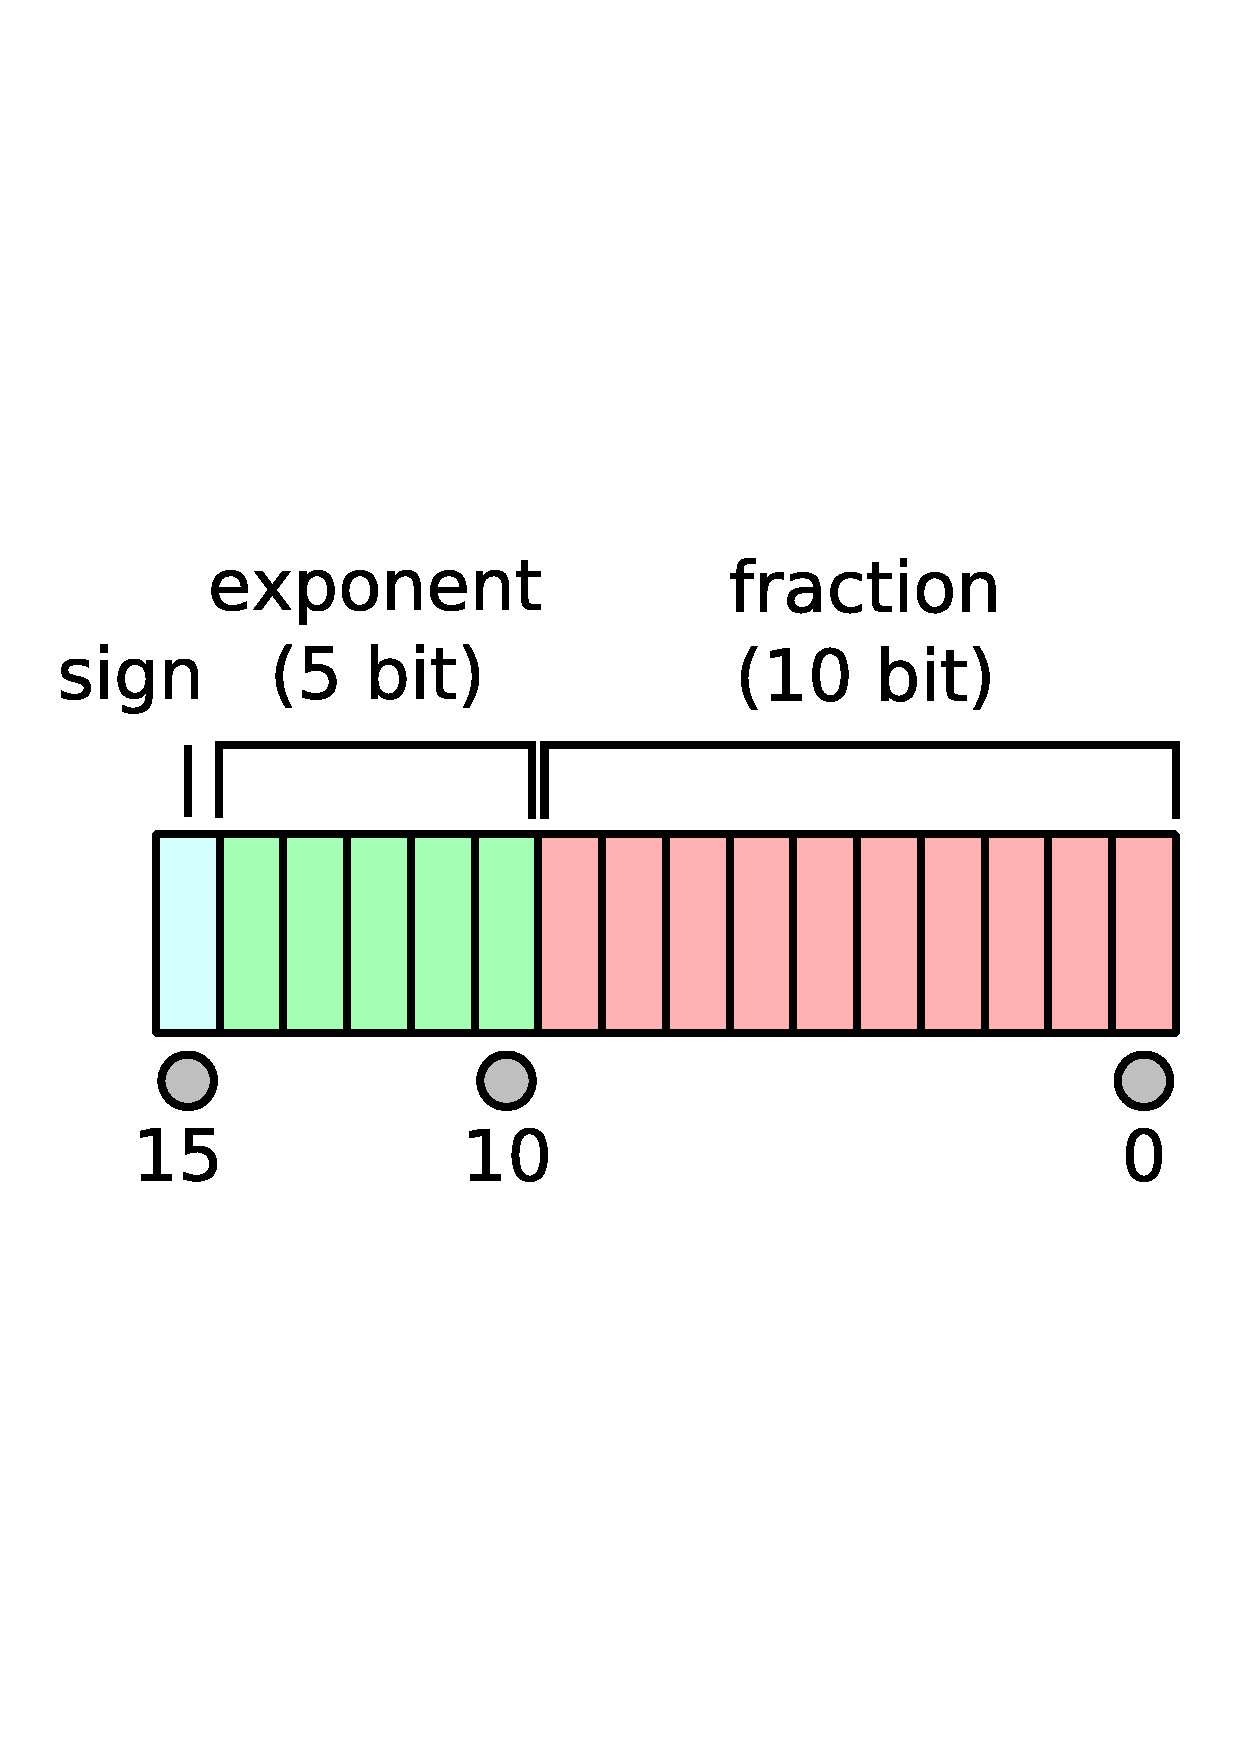
\includegraphics[width=0.4\textwidth]{assets/imgs/half}
\caption{IEEE半精度浮点数的格式定义}
\end{figure}

HLS提供了半精度浮点数(Half-precision floating point)的支持,其格式包含1个符号位,5个指数位和10个尾数位,共16位。半精度浮点数已经广泛地应用于计算机图形学等领域了。这里的优化实现方法只是将板上BRAM存储的矩阵块都用半精度浮点数声明,不改变输入参数的类型与处理系统中声明的数据类型。在FPGA的计算内核中使用半精度浮点数进行强制类型转换。

经过测试,使用半精度浮点数的GEMM算法可以使用最高达到$Dim=96$的矩阵块。此外,由于半精度浮点数运算使用很少的资源,因此可以令$K$对应的块尺寸变得很大,以充分利用板上的计算资源。

综上,GEMM的优化目标是尽可能地利用FPGA的资源,以部署更大的矩阵块来提高计算效率。使用了这一系列优化方式之后,GEMM自身相对于纯CPU的实现已经取得了很大的加速比。下一节具体描述如何令Caffe运行于Zynq SoC上,并与GEMM加速器相结合。

\section{ARM系统实现}

SoCaffe在处理系统上的工作(如图\ref{fig:socaffe})主要分为三个部分:编译与优化使用硬件加速库、交叉编译Caffe与其他第三方库、生成SD卡文件包。本节的工作主要依赖SDSoC工具,使用其提供的IP核、代码生成来构建与FPGA加速器的通信机制,ARM GNU工具链构建动态链接库和交叉编译,bootgen等工具生成包含比特流的Linux系统镜像等等。

% 链接加速器库
\subsection{构建与使用硬件加速库}

尽管在Caffe中使用GEMM加速库只用调用封装好的硬件加速器入口函数即可,但还有些问题需要考虑。首先,GEMM加速器并不适合全部形状的矩阵参数:当矩阵尺寸比较小时,使用GEMM加速器甚至比软件版本慢很多,主要原因是GEMM加速器的额外开销与计算对小尺寸矩阵计算时间而言是显著的。其次,在执行GEMM硬件加速函数的同时,CPU也应该利用起来,进行一些内存分配和复制等等简单操作,这就要求对GEMM硬件函数的调用代码需要异步执行。最后,GEMM硬件加速库与一般软件库不同,其中包含了一个硬件的比特流,选择何时加载、如何加载比特流也是需要考虑的问题。接下来会逐一讨论如何构建与使用GEMM硬件加速库。

\subsubsection{PS-PL接口生成}
调用GEMM加速器函数时,会以处理系统分配好的内存地址作为参数,SDSoC主要根据参数对应的内存块的分配方式来确定生成什么样的接口。如果内存块是以\texttt{malloc}分配生成的,则SDSoC使用Scatter-Gatter类型的接口访问内存中的数据。如果内存块以\texttt{sds\_alloc}分配,则SDSoC可以认识到该内存块是地址连续的,因此会使用顺序访问的接口(比如AXIDMA\_SIMPLE)。除此以外,如果不需要保证缓存的数据一致性,可以指定SDSoC生成使用AFI端口的高速访问数据通路,否则SDSoC会自动使用ACP端口。

\subsubsection{调用方式与条件}

在进行GEMM计算的同时,CPU端往往处于空闲状态。如果此时可以进行一些比较耗时的操作,比如复制数据到矩阵块缓冲区等等,那么系统性能可以得到不错的提升。SDSoC提供了预编译指令\texttt{async <ID>},用来标识硬件函数需要被异步调用;同时也提供了\texttt{wait <ID>}指令来指定等待硬件函数完成的时间点;其中\texttt{<ID>}用来对异步调用任务进行标记。这种异步机制本质上而言构建了FPGA与CPU之间的流水线,提高了系统的并行度。

\begin{listing}[!ht]
\inputminted[
  mathescape, 
  linenos,
  numbersep=5pt,
  breaklines=true,
  fontsize=\footnotesize]{c++}{assets/codes/caffegemm.cpp}

\caption{\texttt{caffe\_cpu\_gemm}函数}
\label{lst:caffegemm}
\end{listing}

正如本节序言所述,GEMM加速器是针对固定大小的矩阵块实现的,因此无法根据输入矩阵的形状进行调整。尤其是当输入矩阵形状非常不规律时,比如一条边很短(~10)而另一些边很长(>1000)时,使用GEMM加速器会带来非常大的性能损耗。本研究使用一种简单条件来判断是否应该执行GEMM:只有当输入矩阵的三个尺寸都大于128时才调用GEMM加速器(如代码\ref{lst:caffegemm}所示,其中当定义了\texttt{SDS}时才会编译\texttt{gemm\_sds}接口),否则使用CPU端的BLAS库。根据测试结果,这种启发式的策略产生了不错的效果,Caffe的性能基本不受矩阵形状的影响了。

\subsubsection{链接库生成}

传统的Zynq SoC应用开发在完成硬件函数的设计之后,是无法使用类似于软件方式调用该硬件逻辑的:必须要通过配置AXI总线的数据并传输数据才能执行硬件逻辑。但使用SDSoC进行开发时却可以直接调用硬件函数,究其原因,主要是因为SDSoC在编译过程中对原始的硬件函数进行了封装,并将封装后的版本替换了原始的函数调用。封装的函数包含了额外的数据准备,信号传输与等待命令完成等一系列过程。正因为如此,SDSoC可以为FPGA硬件逻辑自动构造出一个软件动态链接库。

但硬件逻辑的比特流却不包含在动态链接库中,而是放在一个独立的数据文件中。比特流文件可以在系统引导的过程中加载,也可以在系统运行过程使用\texttt{xdevcfg}设备动态配置。

% 交叉编译
\subsection{交叉编译}

所谓交叉编译,指的是一种编译出来的程序是运行在其他环境中的编译过程。SDSoC中提供的ARM GNU工具链就是在x86环境中交叉编译出ARM环境中可执行代码的交叉编译工具。使用该工具链编译GEMM硬件加速库,以及Caffe本身都很简便,但是涉及到Caffe的第三方库依赖便会遇到很多问题。针对第三方库的交叉编译主要有三种策略:

\begin{enumerate}
\item 直接修改环境变量中的\texttt{CC},\texttt{LD}等为ARM GNU工具链中对应的工具,可以用来处理比较简单的库的编译;
\item 使用第三方库提供的配置方案进行交叉编译配置:大部分第三方库都会使用configure、CMake等工具生成\texttt{Makefile},以方便交叉编译; OpenBLAS在编译工具链的配置之外也会要求指定对应系统架构的名称,进而可以充分优化性能。
\item 其他:有的第三方库完全不支持交叉编译,主要原因是编译过程需要得到编译结果测试的反馈。比如HDF5在编译的过程中,会调用编译出来的程序来生成与目标系统相关的代码,处理起来非常麻烦。
\end{enumerate}

因为第三方库的交叉编译标准不一,而且目标环境相对固定,因此本研究提供一套已经编译好的第三方动态链接库供SoCaffe使用,不需要重复编译,直接链接即可运行。

% 其他细节
\subsection{系统生成}

系统生成过程需要得到最终的、可用的SoCaffe系统,其中要包含编译好的动态链接库,FPGA比特流,以及其他工具等等。本研究按照如下流程构建SoCaffe系统:

\begin{enumerate}
\item 编译硬件加速器动态链接库(\texttt{libaccel.so}),生成包含FPGA比特流的SD卡与相应的引导文件;
\item 编译Caffe链接库(\texttt{libcaffe.so}),并链接第三方库函数和硬件加速器函数;
\item 编译使用SoCaffe环境的代码,比如各种基于Caffe的深度学习应用等等;
\item 将所有生成的链接库,可执行程序复制到第一步生成的SD卡目录中,进而复制到Zynq SoC使用的SD卡;
\item 启动系统,将链接库复制到系统库目录下(\texttt{/lib}),运行需要执行的程序;
\end{enumerate}

\section{总结}

(暂无)
	\chapter{实验结果与分析}

本章对SoCaffe的性能进行测试,首先给出GEMM加速器的独立测试结果,接着给出综合的SoCaffe性能测试。

GEMM测试主要包含GEMM设计过程中的各种优化策略的对比,并且从硬件资源使用和性能两个角度分析。此外,通过GEMM硬件版本与OpenBLAS的CPU版本的不同矩阵块尺寸下的对比,分析得到Caffe调用GEMM硬件操作的最佳时机。

综合SoCaffe测试分别测试了功能的完整性、计算速度与二者的综合。功能的完整性通过Caffe自带的单元测试进行分析;之后使用修改过的\texttt{convnet-benchmarks}\footnote{\url{https://github.com/pku-ceca-research/convnet-benchmarks}}作为基准进行卷积层的性能测试;最终,使用MNIST这一应用对SoCaffe进行整体评估。

\section{实验环境}

\begin{figure}[!ht]
	\centering	
	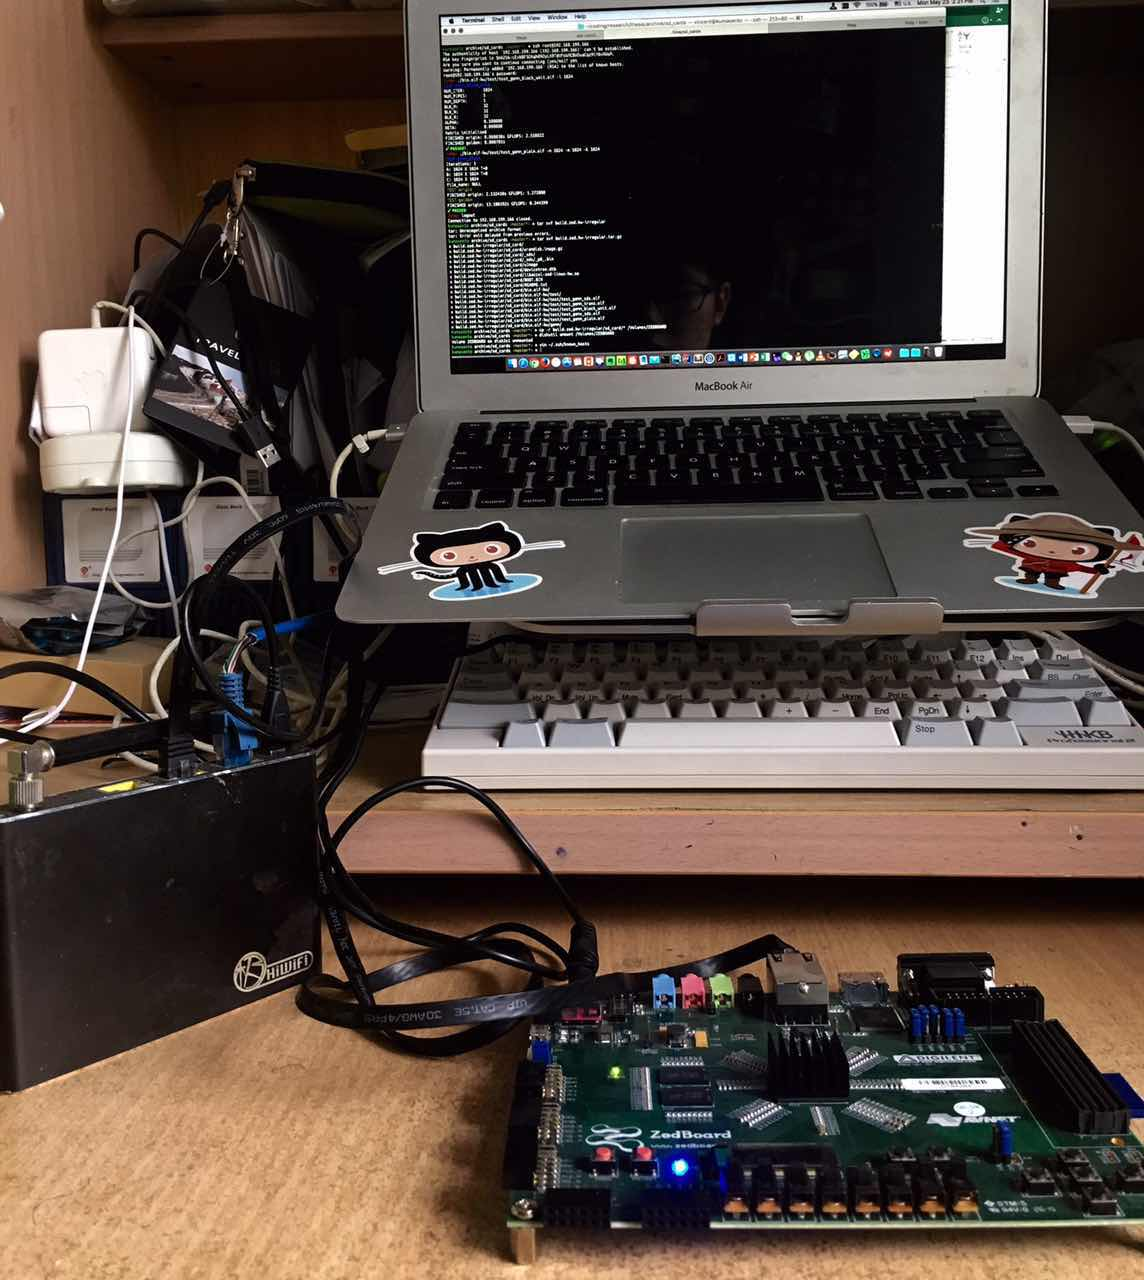
\includegraphics[width=0.6\textwidth]{assets/imgs/env.jpg}
	\caption{实验环境}
	\label{fig:env}
\end{figure}

本研究的实验环境如图\ref{fig:env}所示:Zedboard接上电源后与路由器LAN口通过以太网线连接,WAN口接入有线广域网,主机通过无线网络连接到路由器。配置路由器,令其分配给Zedboard一个固定的ip地址。之后主机即可通过ssh连接Zedboard进行测试。此外,所有的开发与编译过程都在ceca3主机完成,使用2015年4月推出的SDSoC开发平台。

\section{GEMM测试}

\subsection{优化策略对比}\label{subsec:compare}

根据\ref{subsec:gemmopt}节,以及加上\ref{subsubsec:normal},得到如下五个版本实现:原始实现(Baseline)、优化延迟(Latency)、资源分配优化(ResAlloc)、矩阵尺寸优化(IrrShape)以及半精度浮点数优化(HalfFloat)四个版本。本节选取四个版本的设计在最优参数配置下得到的实现作为对比样本,对比的项目包括:
\begin{enumerate}
\item 矩阵尺寸:根据目标版本,能得到的最优的矩阵尺寸;
\item FPGA资源利用:BRAM,DSP,LUT等指标所占用的百分比;
\item 延迟与时钟频率:时钟频率选用能综合得到的最快的时钟频率;
\item 预测性能与实际性能:用GFLOPS作为性能指标;
\end{enumerate}

% 实际性能测试
对实际性能的测试分为两种:GFLOPS块测试与完整测试:GFLOPS块测试只测试对一个GEMM固定矩阵块的计算时间,而GFLOPS完整测试的目标是\texttt{gemm\_sds}的时间,即测试任意大小矩阵的GEMM计算。

\begin{figure}[!ht]
	\centering	
	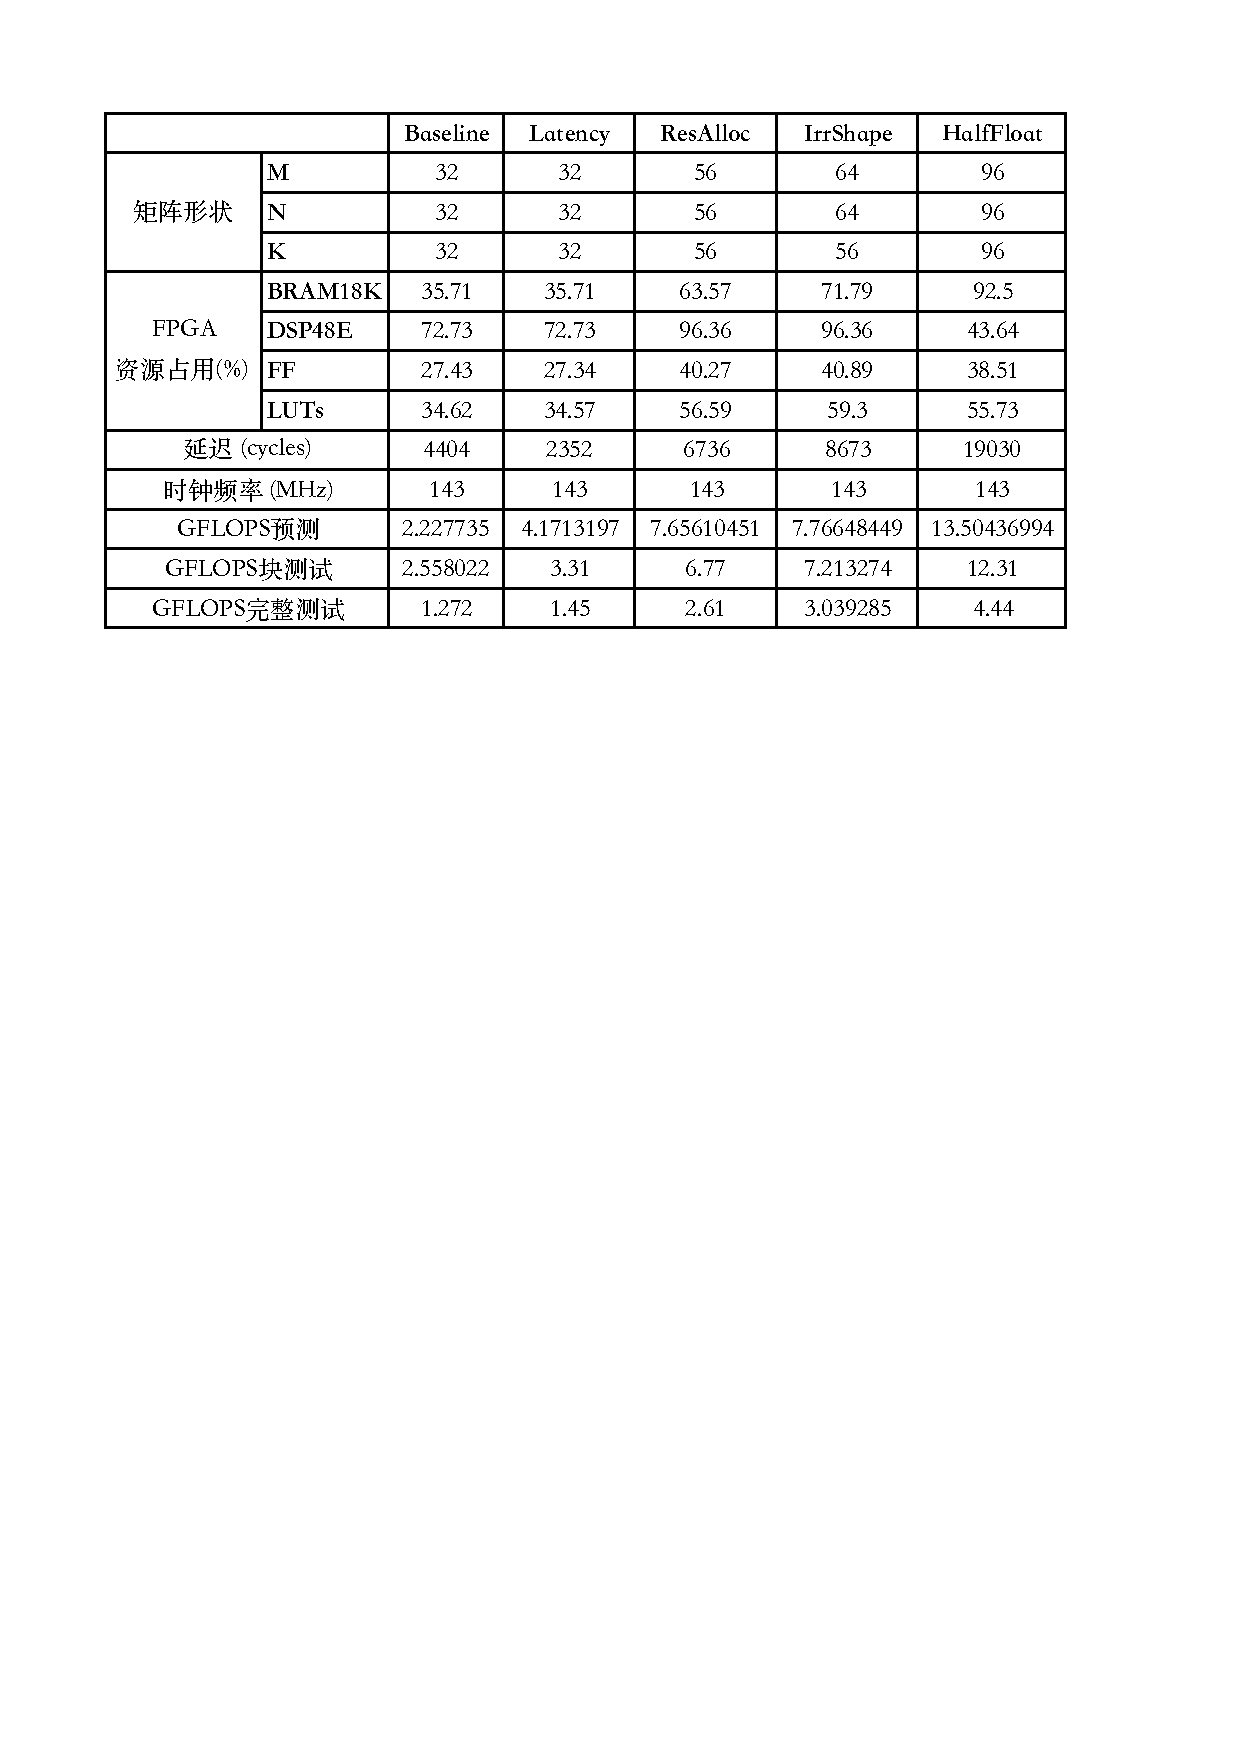
\includegraphics[width=\textwidth]{assets/imgs/gemmcomp.pdf}
	\caption{GEMM优化策略对比结果}
	\label{fig:gemmopt}
\end{figure}

对比结果参见图\ref{fig:gemmopt}。可以发现最快的优化版本是使用半精度浮点数优化的版本,GFLOPS与矩阵块的大小密切相关。尽管资源分配优化与矩阵尺寸优化在$K$对应的矩阵块尺寸上一致,但因为$M$与$N$的不同造成性能上矩阵尺寸优化略优。此外,发现GFLOPS完整测试的GFLOPS相比于块测试的GFLOPS要小,可以看出CPU端的计算确实比较影响最终的计算性能。

\subsection{OpenBLAS对比测试}

OpenBLAS是非常成熟的BLAS计算库,而且也是Caffe兼容的BLAS库之一,因此其在ARM CPU上的运行时间可以作为GEMM硬件加速比的计算基准。

\begin{figure}[!ht]
\centering	
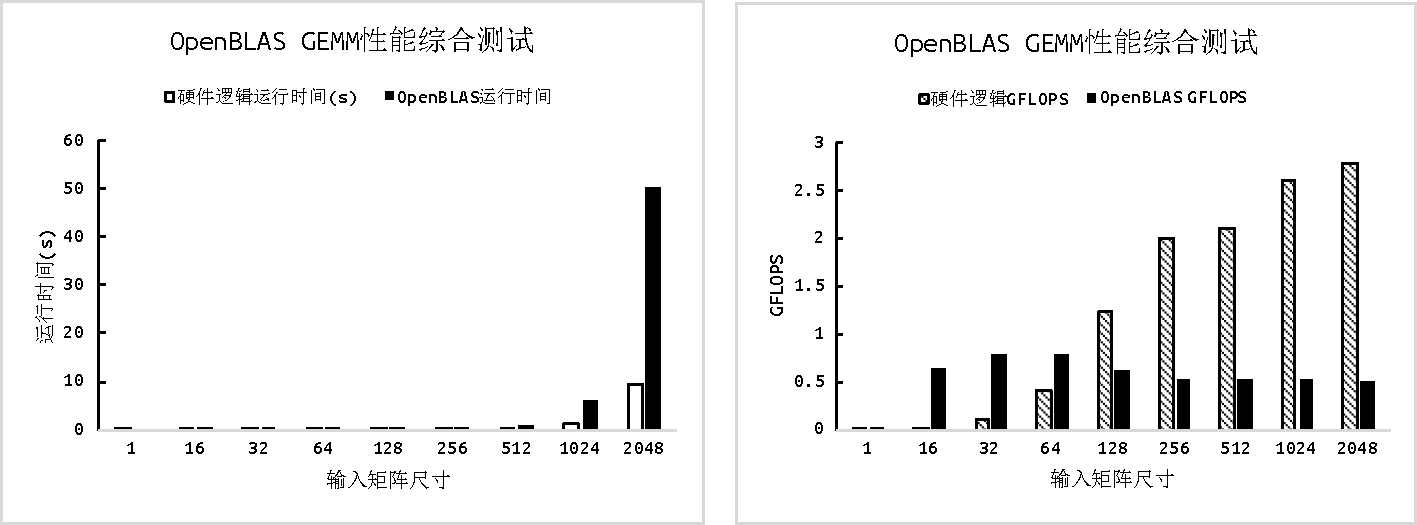
\includegraphics[width=\textwidth]{assets/imgs/gemmblas.pdf}
\caption{GEMM与OpenBLAS的性能对比}
\label{fig:gemmblas}
\end{figure}

这里测试使用的是GEMM在单精度浮点数精度下最快的版本(IrrShape)。与OpenBLAS在多种矩阵尺度下相比,GEMM硬件加速版本确实在小尺寸矩阵上速度很慢,但随着矩阵尺度大于128时,GEMM硬件加速比越来越大。最终测试结果显示GEMM的硬件加速版本是OpenBLAS的5.42倍。

此外,OpenBLAS对比测试与GEMM的完整测试都假定输入矩阵的尺寸一致。这种形式的输入对GEMM的分块计算很友好,很难出现划分不均匀的情况。但是实际中大部分矩阵形态都是不规则的,当划分矩阵块不均匀时,会造成额外的计算并降低性能。但是一般情况下,当矩阵尺寸本身比较大时,额外计算占比不多,对最终性能的影响也不十分显著。

\section{Caffe测试}

\subsection{单元测试}

Caffe的单元测试使用Google Test测试框架\footnote{Google Test\url{(https://github.com/google/googletest)}是一套基于C++的测试框架,提供完整的单元测试(xUnit)搭建功能。}进行搭建,在功能性测试的基础上也加上简单的对性能的测试。

经过运行Caffe的单元测试可以发现,几乎全部的测试都可以通过。但是对于少部分IO测试和HDF5的功能测试出现了问题。初步排查发现是Caffe的单元测试实现问题:部分数据文件在转换到ARM平台以后会无法读写。这类问题在使用lmdb的时候也出现过,需要重新生成一遍文件才能正常读取。由于大部分功能,尤其是关键的深度学习计算功能是完整的且没有问题的,因此本研究先将上述问题搁置,留待后续处理。

\subsection{卷积神经网络性能测试}

\begin{listing}[!ht]
\begin{minted}[
  mathescape, 
  linenos,
  numbersep=5pt,
  breaklines=true,
  fontsize=\footnotesize]{proto}
name: "ConvLayer_3x96x11x11"
input: "data"
input_dim: 32
input_dim: 3
input_dim: 32
input_dim: 32
force_backward: true
layers {
  name: "conv1"
  type: CONVOLUTION
  bottom: "data"
  top: "conv1"
  blobs_lr: 1
  blobs_lr: 2
  convolution_param {
    num_output: 96
    kernel_size: 11
    stride: 1
    weight_filler {
      type: "xavier"
    }
    bias_filler {
      type: "constant"
    }
  }
}
\end{minted}

\caption{卷积层性能测试Caffe网络文件}
\label{lst:convtest}
\end{listing}

由于本研究主要优化了卷积神经网络中需要用到的GEMM计算,因此这里对GEMM于Caffe的融合程度进行测试,观察Caffe的卷积层是否有不错的性能提升。

这里的测试用例使用的网络配置文件为\ref{lst:convtest},根据列举出的参数可以计算得传给GEMM的参数分别为$M=96$,$N=484$,$K=363$(forward计算,backword计算矩阵规模基本一致)。

使用\ref{subsec:compare}中出现的几个设计进行分别测试,基准是OpenBLAS实现的软件版本。测试数据使用Caffe的\texttt{time}指令得到,指定迭代次数为10次:
\begin{figure}[!ht]
	\centering	
	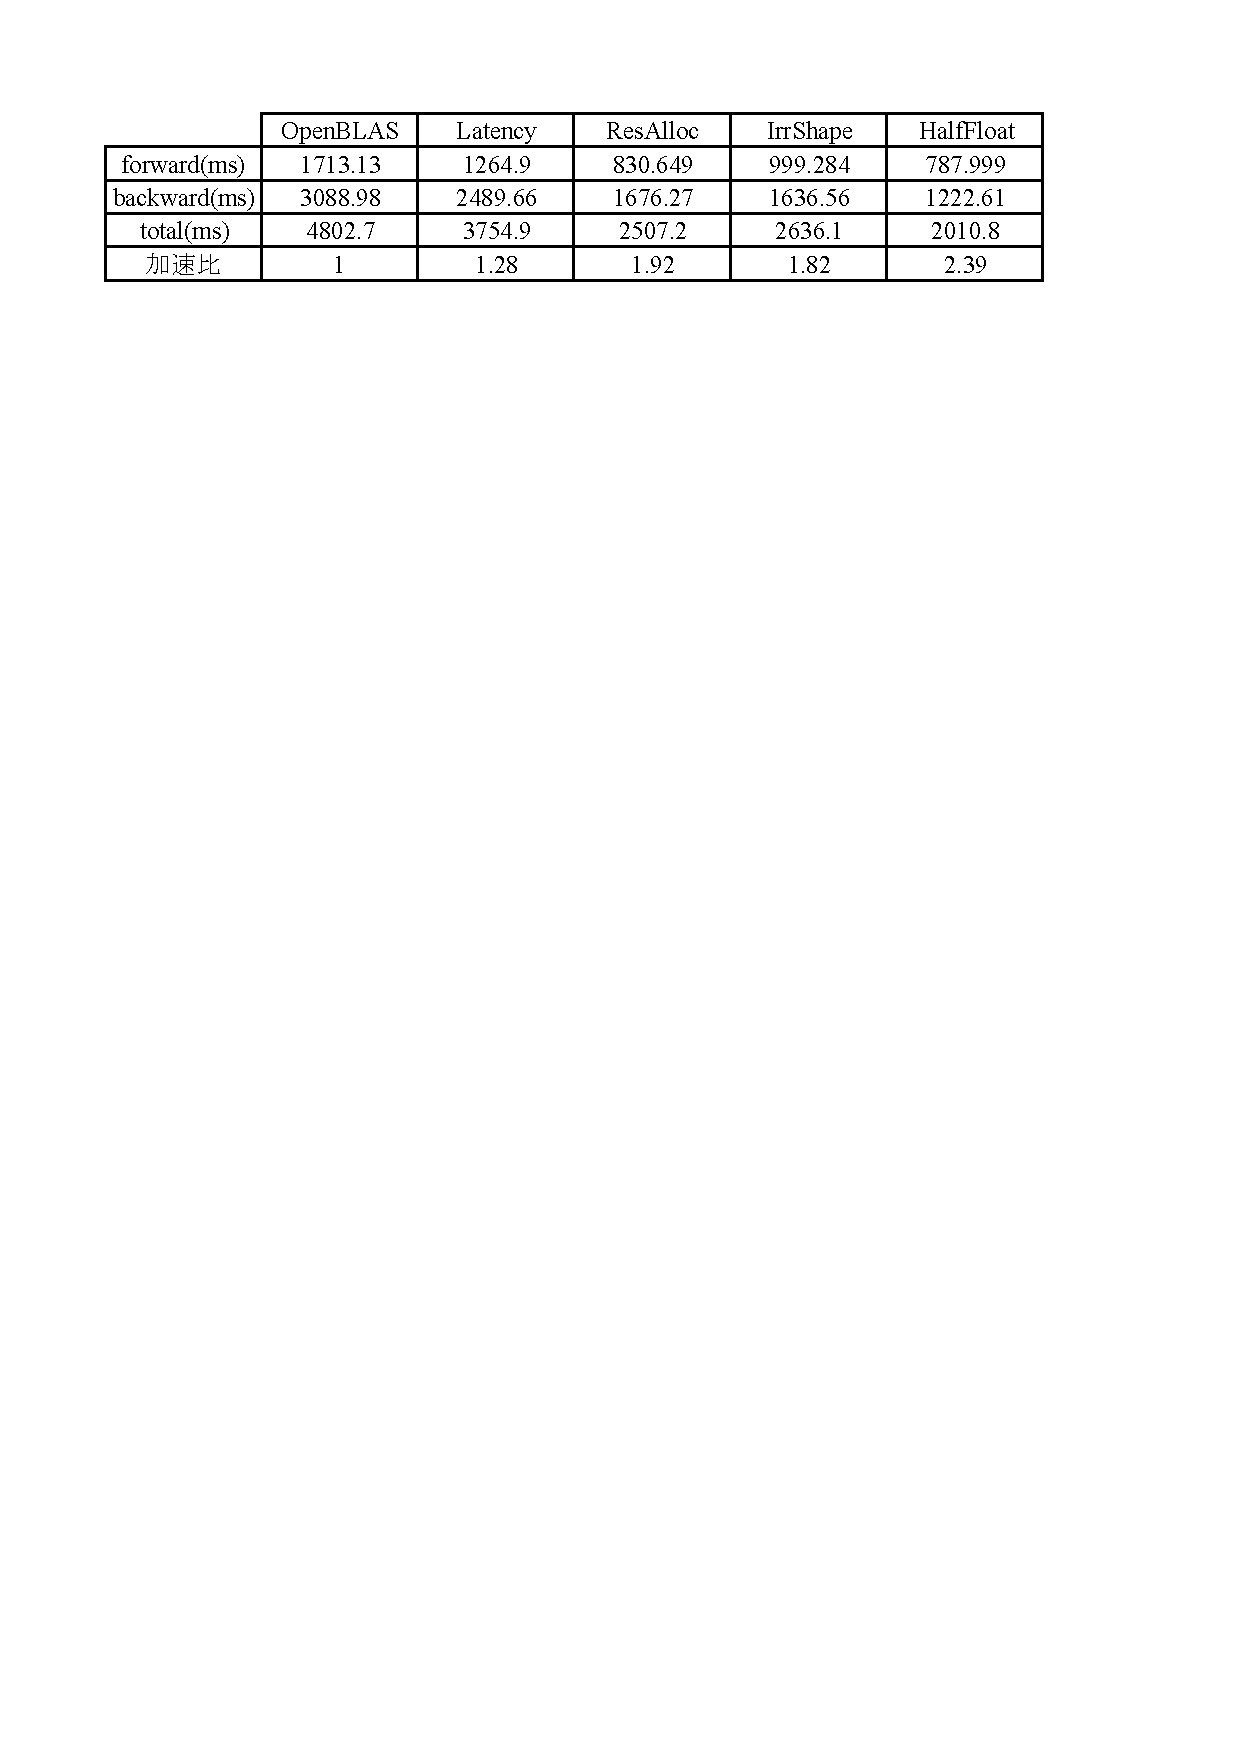
\includegraphics[width=\textwidth]{assets/imgs/caffeconv.pdf}
	\caption{Caffe的卷积层性能测试}
	\label{fig:caffeconv}
\end{figure}

表中的forward与backward分别为计算的前向与反向两个过程,根据结果可以发现最终加速比最高的来自于使用半精度浮点数的版本,达到2.39x。考虑到本测试用例使用的输入矩阵形状不规则,并且结合GEMM的独立测试的数据(\ref{fig:gemmopt}中半精度浮点数的完整测试GFLOPS为4.44),得到上述加速比基本合理。

\subsection{MNIST测试}

MNIST(Mixed National Institute of Standards and Technology)数据集包含大量手写字迹图片数据,常用作对机器学习算法的测试。LeNet\supercite{lecun1998gradient}是基于MNIST一种神经网络结构,因为它的网络结构比较小,并且包含了卷积层、池化层、全连接层和ReLU层,在网络层类型上也比较完整,所以本研究选用MNIST作为真实案例进行测试。

MNIST实现起来很简单,根据Caffe官方教程即可轻易搭建\footnote{\url{http://caffe.berkeleyvision.org/gathered/examples/mnist.html}}。由于在板上训练耗费内存较多,而且效率不高,因此训练过程在GPU主机完成,之后把训练结果复制到板上使用。

MNIST测试主要包含两个部分:性能测试与精度测试,性能测试使用\texttt{time}命令,精度测试使用\texttt{test}搭配之前的训练结果使用。得到的测试结果图\ref{fig:mnist}所示。

在\ref{fig:caffeconv}中表现优异的半精度浮点数的设计在MNIST网络中效率最低,主要是因为设置的96大小的矩阵块会在MNIST网络中造成过多的额外计算。表现最好的是Latency版本,但是与原始的OpenBLAS实现都相差不大。精度测试结果反映出所有的实现都拥有与标准实现一致的准确率,半精度浮点测试也如此,尽管半精度浮点数确实与单精度浮点数相比存在一定的误差。

\begin{figure}[!ht]
	\centering	
	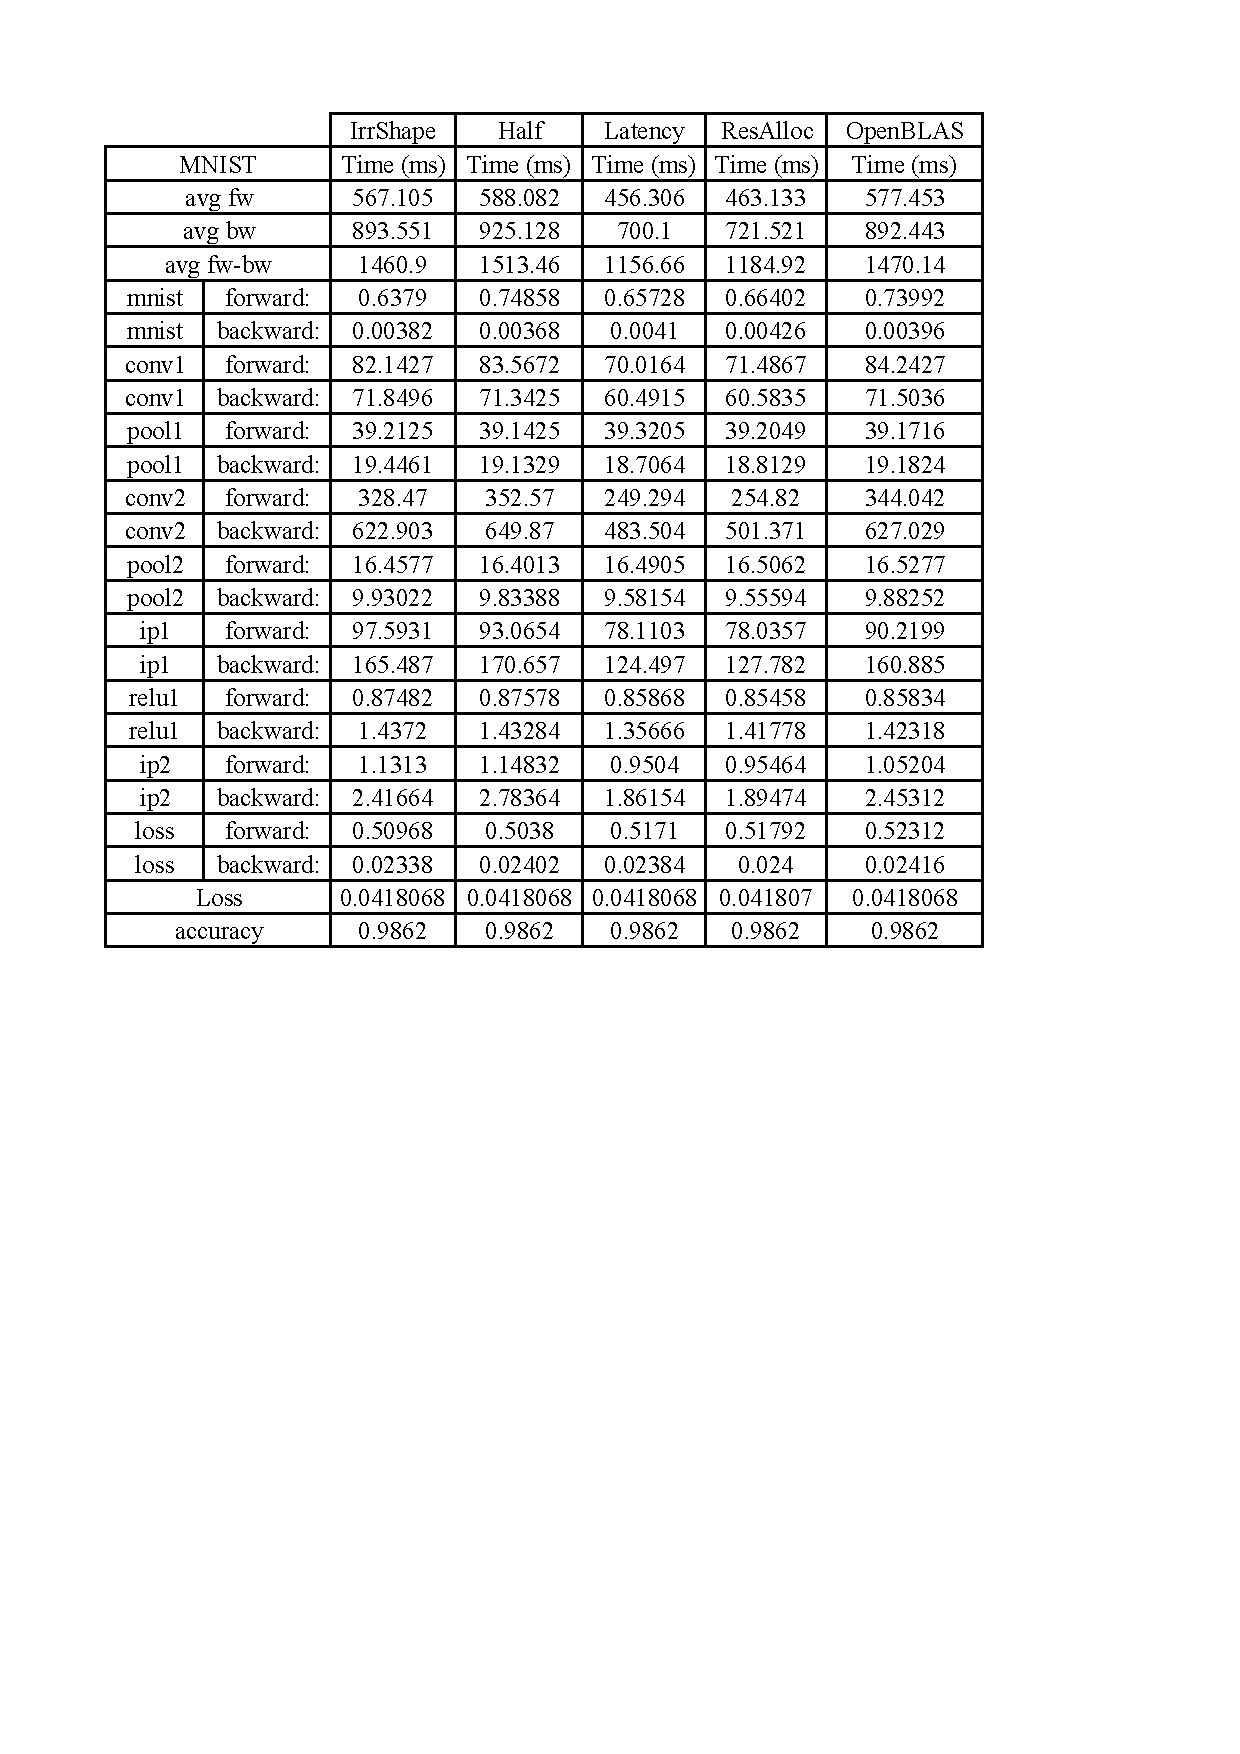
\includegraphics[width=\textwidth]{assets/imgs/mnist.pdf}
	\caption{MNIST网络性能与精度测试}
	\label{fig:mnist}
\end{figure}

总之,MNIST测试的结果主要反映出对于小规模的网络,加速比确实不够明显,而且并不是矩阵块越大效率越高:小规模的网络中额外计算占据的时间比更高。此外,半精度浮点数至少对于MNIST网络而言是完全没有准确率问题。其他网络在使用之前应先测试准确率。
	% 结论。
	% Copyright (c) 2014,2016 Casper Ti. Vector
% Public domain.

\specialchap{结论}

本研究采用了Xilinx公司推出的Zynq-7000全可编程SoC平台,结合深度学习框架Caffe,设计并实现了SoCaffe这一针对嵌入式平台的深度学习框架。最终实现的SoCaffe系统充分利用了Zynq平台的特点,可编程逻辑上实现的GEMM加速算法占用了大部分的硬件资源,基本取得了极限的性能;处理系统部分编译改善了Caffe工具,保持了与Caffe一致的使用方式。因此SoCaffe是一个针对Zynq SoC平台的实际可用的深度学习框架。

本研究的主要工作如下:
\begin{enumerate}
	\item 使用Vivado HLS工具实现了GEMM计算在FPGA上的设计与实现,针对Zynq-7000的系统资源特点给出了相应的优化方案与数学分析模型,找到了能实现的矩阵块大小的上界;同时使用了半精度浮点数优化了对计算资源的使用。最终获得最高12.31GFLOPS和5.42倍加速比。
	\item 系统地学习和掌握了Xilinx SDSoC开发环境的使用方式,通过文档与探索自主掌握了该工具的高级使用方法,并针对SoCaffe的特点定制了一套开发流程。
	\item 使用ARM GNU工具链使用交叉编译的方式编译了全部Caffe需要使用的第三方库,使用SDSoC构建了SoCaffe的系统镜像文件包和动态链接库。
	\item 测试了SoCaffe的计算性能,可用性,精度等等特性,找到了SoCaffe的最佳使用条件:即针对大量使用卷积神经网络,网络规模较大的时候,SoCaffe可以取得不错的加速比。
\end{enumerate}

此外,SoCaffe也存在一些缺点和亟待提高的地方:首先,因为Zynq SoC平台的内存有限,SoCaffe无法支持特别大的神经网络结构;其次,SoCaffe的GEMM固定块算法依然有一定的比重是冗余计算,如果输入矩阵形状比较小,则会造成较大比例的性能损失;最后,SoCaffe目前只支持GEMM的优化,其他不用到GEMM操作的网络层不能得到相应的性能提升。这些工作都是本研究下一步要进行优化的工作。



% vim:ts=4:sw=4


	% 正文中的附录部分。
	\appendix
	% 排版参考文献列表。bibintoc 选项使“参考文献”出现在目录中;
	% 如果同时要使参考文献列表参与章节编号,可将“bibintoc”改为“bibnumbered”。
	\printbibliography[heading = bibintoc]
	% 各附录。
	% % Copyright (c) 2014,2016 Casper Ti. Vector
% Public domain.

\chapter{附件}

\section{测试结果}
\begin{figure}[!ht]
	\centering	
	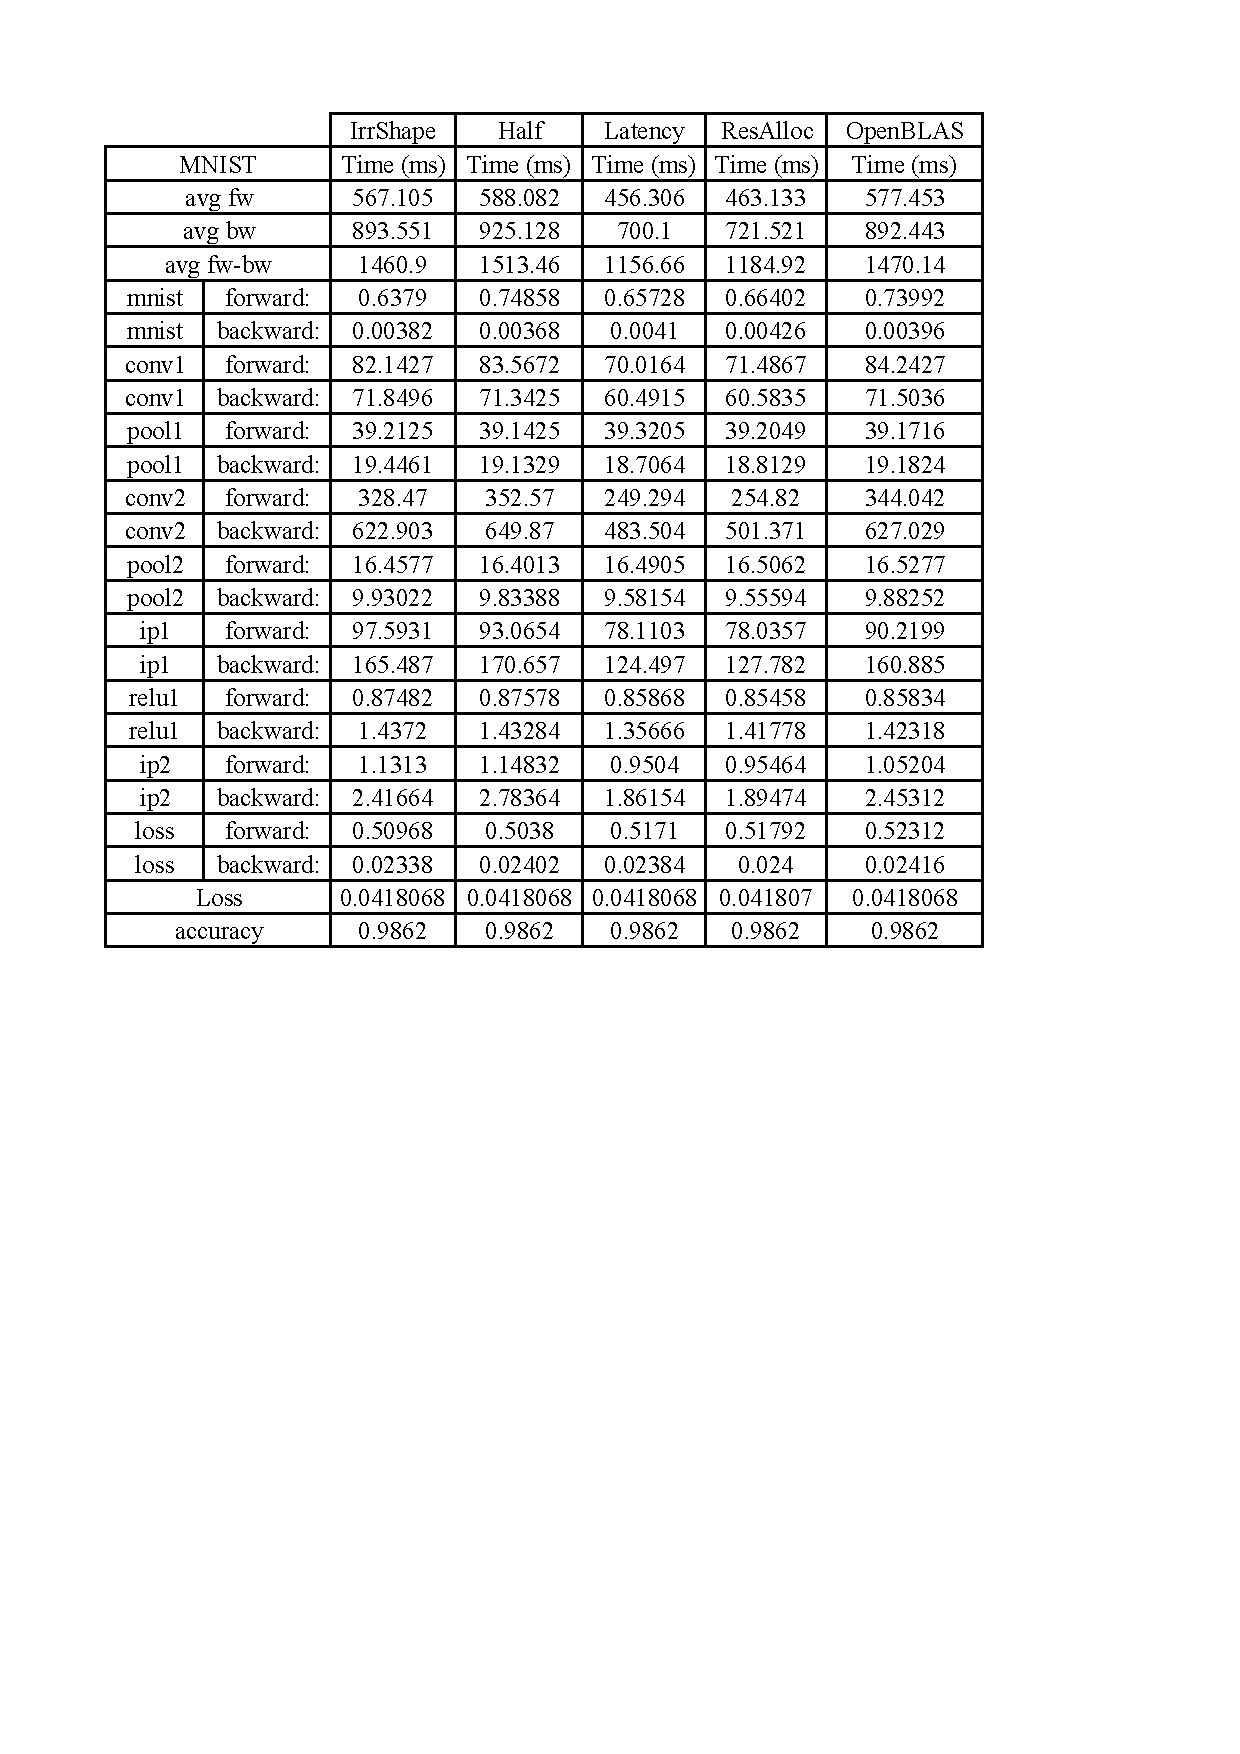
\includegraphics[width=\textwidth]{assets/imgs/mnist.pdf}
	\caption{MNIST网络性能与精度测试}
	\label{fig:mnist}
\end{figure}


% vim:ts=4:sw=4


	% 以下为正文之后的部分,默认不进行章节编号。
	\backmatter
	% 致谢。
	% Copyright (c) 2014,2016 Casper Ti. Vector
% Public domain.

\chapter{致谢}
\pkuthssffaq % 中文测试文字。

% vim:ts=4:sw=4

	% 原创性声明和使用授权说明。
	% Copyright (c) 2008-2009 solvethis
% Copyright (c) 2010-2016 Casper Ti. Vector
% All rights reserved.
%
% Redistribution and use in source and binary forms, with or without
% modification, are permitted provided that the following conditions are
% met:
%
% * Redistributions of source code must retain the above copyright notice,
%   this list of conditions and the following disclaimer.
% * Redistributions in binary form must reproduce the above copyright
%   notice, this list of conditions and the following disclaimer in the
%   documentation and/or other materials provided with the distribution.
% * Neither the name of Peking University nor the names of its contributors
%   may be used to endorse or promote products derived from this software
%   without specific prior written permission.
%
% THIS SOFTWARE IS PROVIDED BY THE COPYRIGHT HOLDERS AND CONTRIBUTORS "AS
% IS" AND ANY EXPRESS OR IMPLIED WARRANTIES, INCLUDING, BUT NOT LIMITED TO,
% THE IMPLIED WARRANTIES OF MERCHANTABILITY AND FITNESS FOR A PARTICULAR
% PURPOSE ARE DISCLAIMED. IN NO EVENT SHALL THE COPYRIGHT HOLDER OR
% CONTRIBUTORS BE LIABLE FOR ANY DIRECT, INDIRECT, INCIDENTAL, SPECIAL,
% EXEMPLARY, OR CONSEQUENTIAL DAMAGES (INCLUDING, BUT NOT LIMITED TO,
% PROCUREMENT OF SUBSTITUTE GOODS OR SERVICES; LOSS OF USE, DATA, OR
% PROFITS; OR BUSINESS INTERRUPTION) HOWEVER CAUSED AND ON ANY THEORY OF
% LIABILITY, WHETHER IN CONTRACT, STRICT LIABILITY, OR TORT (INCLUDING
% NEGLIGENCE OR OTHERWISE) ARISING IN ANY WAY OUT OF THE USE OF THIS
% SOFTWARE, EVEN IF ADVISED OF THE POSSIBILITY OF SUCH DAMAGE.

{
	\CTEXsetup[
		format+ = {\centering}, beforeskip = {40bp}, afterskip = {15bp}
	]{section}

	% 学校书面要求本页面不要页码,但在给出的 Word 模版中又有页码且编入了目录。
	% 此处以 Word 模版为实际标准进行设定。
	\specialchap{北京大学学位论文原创性声明和使用授权说明}
	\mbox{}\vspace*{-3em}
	\section*{原创性声明}

	本人郑重声明:
	所呈交的学位论文,是本人在导师的指导下,独立进行研究工作所取得的成果。
	除文中已经注明引用的内容外,
	本论文不含任何其他个人或集体已经发表或撰写过的作品或成果。
	对本文的研究做出重要贡献的个人和集体,均已在文中以明确方式标明。
	本声明的法律结果由本人承担。
	\vskip 1em
	\rightline{%
		论文作者签名:\hspace{5em}%
		日期:\hspace{2em}年\hspace{2em}月\hspace{2em}日%
	}

	\section*{%
		学位论文使用授权说明\\[-0.33em]
		\textmd{\zihao{5}(必须装订在提交学校图书馆的印刷本)}%
	}

	本人完全了解北京大学关于收集、保存、使用学位论文的规定,即:
	\begin{itemize}
		\item 按照学校要求提交学位论文的印刷本和电子版本;
		\item 学校有权保存学位论文的印刷本和电子版,
			并提供目录检索与阅览服务,在校园网上提供服务;
		\item 学校可以采用影印、缩印、数字化或其它复制手段保存论文;
		\item 因某种特殊原因需要延迟发布学位论文电子版,
			授权学校在 $\Box$\nobreakspace{}一年 /
			$\Box$\nobreakspace{}两年 /
			$\Box$\nobreakspace{}三年以后在校园网上全文发布。
	\end{itemize}
	\centerline{(保密论文在解密后遵守此规定)}
	\vskip 1em
	\rightline{%
		论文作者签名:\hspace{5em}导师签名:\hspace{5em}%
		日期:\hspace{2em}年\hspace{2em}月\hspace{2em}日%
	}

	% 若需排版二维码,请将二维码图片重命名为“barcode”,
	% 转为合适的图片格式,并放在当前目录下,然后去掉下面 2 行的注释。
	%\vfill\noindent
	%\includegraphics[height = 5em]{barcode}
}

% vim:ts=4:sw=4

\end{document}

% vim:ts=4:sw=4
